\documentclass[
	% -- opções da classe memoir --
	12pt,				% tamanho da fonte
	openright,			% capítulos começam em pág ímpar (insere página vazia caso preciso)
	oneside,			% para impressão em verso e anverso. Oposto a oneside
	a4paper,			% tamanho do papel. 
	% -- opções da classe abntex2 --
	%chapter=TITLE,		% títulos de capítulos convertidos em letras maiúsculas
	%section=TITLE,		% títulos de seções convertidos em letras maiúsculas
	%subsection=TITLE,	% títulos de subseções convertidos em letras maiúsculas
	%subsubsection=TITLE,% títulos de subsubseções convertidos em letras maiúsculas
	% -- opções de sumário -- %
	sumario=abnt-6027-2012, % sumário conforme as recomendações da ABNT NBR 6027:2012 (padrão)
	%sumario=tradicional, % usa o estilo tradicional de sumários do memoir
	.
	% -- opções do pacote babel --
	english,			% idioma adicional para hifenização
	brazil				% o último idioma é o principal do documento
	]{abntex2}


% --- 
% CONFIGURAÇÕES DE PACOTES
% --- 
% ---
% Pacotes básicos 
% ---
\usepackage{lmodern}			% Usa a fonte Latin Modern			
\usepackage[T1]{fontenc}		% Selecao de codigos de fonte.
\usepackage[utf8]{inputenc}		% Codificacao do documento (conversão automática dos acentos)
\usepackage{lastpage}			% Usado pela Ficha catalográfica
\usepackage{indentfirst}		% Indenta o primeiro parágrafo de cada seção.
\usepackage{color}				% Controle das cores
\usepackage{graphicx}			% Inclusão de gráficos
\usepackage{microtype} 			% para melhorias de justificação
\usepackage{ufc-abntex2}

\usepackage{amsmath}            % Organizar numeração das figuras por seção 
\numberwithin{figure}{chapter}

 \usepackage{tikz}
 \usetikzlibrary{mindmap}
 \usepackage{metalogo}
% \usepackage{dtklogos}

%\usepackage{subfig}
% ---
		
% ---
% Pacotes adicionais, usados apenas no âmbito do Modelo Canônico do abnteX2
% ---
\usepackage{lipsum}				% para geração de dummy text
\usepackage[nolist]{acronym}    % Inclusão de acronimos
% ---

% ---
% Pacotes de citações
% ---
\usepackage[brazilian,hyperpageref]{backref}	 % Paginas com as citações na bibl
\usepackage[alf,abnt-and-type=e,abnt-full-initials=no,abnt-last-names=abnt,abnt-etal-list=2,abnt-etal-text = emph,abnt-emphasize=bf]{abntex2cite}
%\usepackage[alf]{abntex2cite}	% Citações padrão ABNT

% ---
% Configurações do pacote backref
% Usado sem a opção hyperpageref de backref
\renewcommand{\backrefpagesname}{Citado na(s) página(s):~}
% Texto padrão antes do número das páginas
\renewcommand{\backref}{}
% Define os textos da citação
\renewcommand*{\backrefalt}[4]{
	\ifcase #1 %
		Nenhuma citação no texto.%
	\or\renewcommand{\cftsubsectionfont}{\bfseries\itshape}
	\renewcommand{\cftsubsubsectionfont}{\bfseries}
	
		Citado na página #2.%
	\else
		Citado #1 vezes nas páginas #2.%
	\fi}%
% ---

% ---
% Configurações de aparência do PDF final

%\renewcommand{\cftsubsectionfont}{\bfseries\itshape}
\renewcommand{\cftsubsectionfont}{\itshape}
\renewcommand{\cftsubsubsectionfont}{\itshape}
\renewcommand{\cftsubsubsectionfont}{\cftsubsectionfont}

\newcommand\figref{Figura~\ref}
\newcommand\capref{Capítulo~\ref}
\newcommand\tabref{Tabela~\ref}
\newcommand\secref{Seção~\ref}
% alterando o aspecto da cor azul
\definecolor{blue}{RGB}{41,5,195}

% informações do PDF
\makeatletter
\hypersetup{
     	%pagebackref=true,
		pdftitle={\@title}, 
		pdfauthor={\@author},
    	pdfsubject={\imprimirpreambulo},
	    pdfcreator={LaTeX with abnTeX2},
		pdfkeywords={abnt}{latex}{abntex}{abntex2}{trabalho acadêmico}, 
		colorlinks=true,       		% false: boxed links; true: colored links
    	linkcolor=black,          	% color of internal links
    	citecolor=black,        		% color of links to bibliography
    	filecolor=black,      		% color of file links
		urlcolor=black,
		bookmarksdepth=4
}
\makeatother
% --- 

% Definições matemáticas
\newcommand{\mean}[1]{\mathbb{E}\left\{ #1 \right\}}
\newcommand{\Abs}[1]{\left\vert #1 \right\vert}
\newcommand{\stK}{\Set{K}}
\usepackage{mathtools}
\usepackage{amssymb,amstext,amsfonts}

% Pacote para tabela
\usepackage{threeparttable}

\usetikzlibrary{arrows.meta}
\tikzset{%
	>={Latex[width=2mm,length=2mm]},
	% Specifications for style of nodes:
	base/.style = {rectangle, rounded corners, draw=black,
		minimum width=4cm, minimum height=1cm,
		text centered, font=\sffamily},
	activityStarts/.style = {base, fill=blue!30},
	startstop/.style = {base, fill=red!30},
	activityRuns/.style = {base, fill=green!30},
	process/.style = {base, minimum width=2.5cm, fill=orange!15,
		font=\ttfamily},
}

% Cross reference
\usepackage{xr}
%acro
\usepackage{acronym}

% --- 
% Espaçamentos entre linhas e parágrafos 
% --- 

% O tamanho do parágrafo é dado por:
\setlength{\parindent}{1.3cm}

% Controle do espaçamento entre um parágrafo e outro:
\setlength{\parskip}{0.2cm}  % tente também \onelineskip

% ---
% compila o indice
% ---
\makeindex
% ---

%\usepackage[xindy={language=portuguese},nonumberlist=true]{glossaries}

% Informações de dados para CAPA e FOLHA DE ROSTO
\titulo{ IMPLEMENTAÇÃO E ANÁLISE DE UM FRAMEWORK DE DETECÇÃO DE ATAQUES DISTRIBUÍDOS DE NEGAÇÃO DE SERVIÇO }
\autor{BRUNO RICCELLI DOS SANTOS SILVA}
\local{Fortaleza, Ceará}
\data{2017}
\orientador{Prof. Msc. Ricardo Jardel Nunes da Silveira}
\coorientador{Prof. Msc. Marcelo Araújo Lima}

\instituicao{%
Universidade Federal do Ceará \\
Centro de Tecnologia \\
Departamento de Engenharia de Teleinformática \par
Curso de Engenharia de Computação
}
\tipotrabalho{Trabalho de Conclusão de Curso (Monografia)}
\preambulo{Monografia apresentada ao Curso de Engenharia de Computação da Universidade Federal do Ceará, como requisito parcial para obtenção do Título de Bacharel em Engenharia de Computação.}

%\newacronym{3GPP}{3GPP}{3rd Generation Partnership Project}
\newacronym{3GPP2}{3GPP2}{3rd Generation Partnership Project 2}
\newacronym{1G}{1G}{1$^\text{st}$~Generation}
\newacronym{2G}{2G}{2$^\text{nd}$~Generation}
\newacronym{3G}{3G}{3$^\text{rd}$~Generation}
\newacronym{4G}{4G}{4$^\text{th}$~Generation}
\newacronym{5G}{5G}{5$^\text{th}$~Generation}
\newacronym{AA}{AA}{Antenna Array}
\newacronym{AC}{AC}{Admission Control}
\newacronym{AD}{AD}{Attack-Decay}
\newacronym{ABS}{ABS}{Almost Blank Subframe}
\newacronym{ADSL}{ADSL}{Asymmetric Digital Subscriber Line}
\newacronym{AHW}{AHW}{Alternate Hop-and-Wait}
\newacronym{AMC}{AMC}{Adaptive Modulation and Coding}
\newacronym{AP}{AP}{Access Point}
\newacronym{APA}{APA}{Adaptive Power Allocation}
\newacronym{ARMA}{ARMA}{Autoregressive Moving Average}
\newacronym{ATES}{ATES}{Adaptive Throughput-based Efficiency-Satisfaction Trade-Off}
\newacronym{AWGN}{AWGN}{Additive White Gaussian Noise}
\newacronym{BB}{BB}{Branch and Bound}
\newacronym{BC}{BC}{Branch and Cut}
\newacronym{BD}{BD}{Block Diagonalization}
\newacronym{BER}{BER}{Bit Error Rate}
\newacronym{BF}{BF}{Best Fit}
\newacronym{BL}{BL}{Bit Loading}
\newacronym{BLER}{BLER}{BLock Error Rate}
\newacronym{BPC}{BPC}{Binary Power Control}
\newacronym{BPSK}{BPSK}{Binary Phase-Shift Keying}
\newacronym{BRA}{BRA}{Balanced Random Allocation}
\newacronym{BS}{BS}{Base Station}
\newacronym{CAP}{CAP}{Combinatorial Allocation Problem}
\newacronym{CAPEX}{CAPEX}{Capital Expenditure}
\newacronym{CBF}{CBF}{Coordinated Beamforming}
\newacronym{CBR}{CBR}{Constant Bit Rate}
\newacronym{CBS}{CBS}{Class Based Scheduling}
\newacronym{CC}{CC}{Congestion Control}
\newacronym{CDF}{CDF}{Cumulative Distribution Function}
\newacronym{CDMA}{CDMA}{Code-Division Multiple Access}
\newacronym{CL}{CL}{Closed Loop}
\newacronym{CLPC}{CLPC}{Closed Loop Power Control}
\newacronym{CNR}{CNR}{Channel-to-Noise Ratio}
\newacronym{CPA}{CPA}{Cellular Protection Algorithm}
\newacronym{CPICH}{CPICH}{Common Pilot Channel}
\newacronym{CoMP}{CoMP}{Coordinated Multi-Point}
\newacronym{CQI}{CQI}{Channel Quality Indicator}
\newacronym{CRA}{CRA}{Capacity-driven Resource Allocation}
\newacronym{CRE}{CRE}{Cell Range Expansion}
\newacronym{CRM}{CRM}{Constrained Rate Maximization}
\newacronym{CRN}{CRN}{Cognitive Radio Network}
\newacronym{CS}{CS}{Coordinated Scheduling}
\newacronym{CSI}{CSI}{Channel State Information}
\newacronym{CTS}{CTS}{Clear to Send}
\newacronym{CUE}{CUE}{Cellular User Equipment}
\newacronym{D2D}{D2D}{Device-to-Device}
\newacronym{DCA}{DCA}{Dynamic Channel Allocation}
\newacronym{DE}{DE}{Differential Evolution}
\newacronym{DF}{DF}{Decode and Forward}
\newacronym{DFT}{DFT}{Discrete Fourier Transform}
\newacronym{DIST}{DIST}{Distance}
\newacronym{DL}{DL}{Downlink}
\newacronym{DMA}{DMA}{Double Moving Average}
\newacronym{DMRS}{DMRS}{Demodulation Reference Signal}
\newacronym{D2DM}{D2DM}{D2D Mode}
\newacronym{DMS}{DMS}{D2D Mode Selection}
\newacronym{DPC}{DPC}{Dirty Paper Coding}
\newacronym{DRA}{DRA}{Dynamic Resource Assignment}
\newacronym{DSA}{DSA}{Dynamic Spectrum Access}
\newacronym{DSM}{DSM}{Delay-based Satisfaction Maximization}
\newacronym{ECC}{ECC}{Electronic Communications Committee}
\newacronym{EE}{EE}{Energy Efficiency}
\newacronym{EFLC}{EFLC}{Error Feedback Based Load Control}
\newacronym{EI}{EI}{Efficiency Indicator}
\newacronym{e-ICIC}{e-ICIC}{Enhanced Inter-Cell Interference Coordination}
\newacronym{eNB}{eNB}{Evolved Node B}
\newacronym{EPA}{EPA}{Equal Power Allocation}
\newacronym{EPC}{EPC}{Evolved Packet Core}
\newacronym{EPS}{EPS}{Evolved Packet System}
\newacronym{E-UTRAN}{E-UTRAN}{Evolved Universal Terrestrial Radio Access Network}
\newacronym{ES}{ES}{Exhaustive Search}
\newacronym{EXP}{EXP}{Exponential}
\newacronym{FCP}{FCP}{Fundamental Counting Principle}
\newacronym{FD}{FD}{Full-Duplex Communications}
\newacronym{FDD}{FDD}{Frequency Division Duplex}
\newacronym{FDM}{FDM}{Frequency Division Multiplexing}
\newacronym{FDMA}{FDMA}{Frequency Division Multiple Access}
\newacronym{FER}{FER}{Frame Erasure Rate}
\newacronym{FF}{FF}{Fast Fading}
\newacronym{FSB}{FSB}{Fixed Switched Beamforming}
\newacronym{FST}{FST}{Fixed SNR Target}
\newacronym{FTP}{FTP}{File Transfer Protocol}
\newacronym{GA}{GA}{Genetic Algorithm}
\newacronym{GAP}{GAP}{Generalized Assignment Problem}
\newacronym{GAP-MQ}{GAP-MQ}{Generalized Assignment Problem with Minimum Quantities}
\newacronym{GBR}{GBR}{Guaranteed Bit Rate}
\newacronym{GLR}{GLR}{Gain to Leakage Ratio}
\newacronym{GOS}{GOS}{Generated Orthogonal Sequence}
\newacronym{GPL}{GPL}{GNU General Public License}
\newacronym{GRP}{GRP}{Grouping}
\newacronym{GTEL}{GTEL}{Wireless Telecommunications Research Group}
\newacronym{GSM}{GSM}{Global System for Mobile Communications}
\newacronym{HARQ}{HARQ}{Hybrid Automatic Repeat Request}
\newacronym{HetNet}{HetNet}{Heterogeneous Network}
\newacronym{HH}{HH}{Hughes-Hartogs}
\newacronym{HMS}{HMS}{Harmonic Mode Selection}
\newacronym{HOL}{HOL}{Head Of Line}
\newacronym{HSDPA}{HSDPA}{High-Speed Downlink Packet Access}
\newacronym{HSPA}{HSPA}{High Speed Packet Access}
\newacronym{HTTP}{HTTP}{HyperText Transfer Protocol}
\newacronym{ICMP}{ICMP}{Internet Control Message Protocol}
\newacronym{ICI}{ICI}{Intercell Interference}
\newacronym{ICIC}{ICIC}{Inter-Cell Interference Coordination}
\newacronym{ID}{ID}{Identification}
\newacronym{IETF}{IETF}{Internet Engineering Task Force}
\newacronym{ILP}{ILP}{Integer Linear Program}
\newacronym{UID}{UID}{Unique Identification}
\newacronym{IID}{IID}{Independent and Identically Distributed}
\newacronym{IIR}{IIR}{Infinite Impulse Response}
\newacronym{IMT}{IMT}{International Mobile Telecommunications}
\newacronym{INV}{INV}{Inverted Norm-based Grouping}
\newacronym{IoT}{IoT}{Internet of Things}
\newacronym{IP}{IP}{Internet Protocol}
\newacronym{IPv6}{IPv6}{Internet Protocol Version 6}
\newacronym{ISD}{ISD}{Inter-Site Distance}
\newacronym{ISI}{ISI}{Inter Symbol Interference}
\newacronym{ISM}{ISM}{Industrial, Scientific and Medical}
\newacronym{ITU}{ITU}{International Telecommunication Union}
\newacronym{JOAS}{JOAS}{Joint Opportunistic Assignment and Scheduling}
\newacronym{JOS}{JOS}{Joint Opportunistic Scheduling}
\newacronym{JP}{JP}{Joint Processing}
\newacronym{JRAPAP}{JRAPAP}{Joint RB Assignment and Power Allocation Problem}
\newacronym{JS}{JS}{Jump-Stay}
\newacronym{JSM}{JSM}{Joint Satisfaction Maximization}
\newacronym{KKT}{KKT}{Karush-Kuhn-Tucker}
\newacronym{LAC}{LAC}{Link Admission Control}
\newacronym{LA}{LA}{Link Adaptation}
\newacronym{LC}{LC}{Load Control}
\newacronym{LOS}{LOS}{Line of Sight}
\newacronym{LP}{LP}{Linear Programming}
\newacronym{LTE}{LTE}{Long Term Evolution}
\newacronym{LTE-A}{LTE-A}{\ac{LTE}-Advanced}
\newacronym{LTE-Advanced}{LTE-Advanced}{Long Term Evolution Advanced}
\newacronym{M2M}{M2M}{Machine-to-Machine}
\newacronym{MAC}{MAC}{Medium Access Control}
\newacronym{MANET}{MANET}{Mobile Ad hoc Network}
\newacronym{MC}{MC}{Modular Clock}
\newacronym{MCS}{MCS}{Modulation and Coding Scheme}
\newacronym{MDB}{MDB}{Measured Delay Based}
\newacronym{MDI}{MDI}{Minimum D2D Interference}
\newacronym{MDSM}{MDSM}{Modified Delay-based Satisfaction Maximization}
\newacronym{MDU}{MDU} {Max-Delay-Utility}
\newacronym{MF}{MF}{Matched Filter}
\newacronym{MG}{MG}{Maximum Gain}
\newacronym{MH}{MH}{Multi-Hop}
\newacronym{MILP}{MILP}{Mixed Integer Linear Problem} %{Mixed Integer Linear Programming}
\newacronym{MIMO}{MIMO}{Multiple Input Multiple Output}
\newacronym{MINLP}{MINLP}{Mixed Integer Nonlinear Programming}
\newacronym{MIP}{MIP}{Mixed Integer Programming}
\newacronym{MISO}{MISO}{Multiple Input Single Output}
\newacronym{MLWDF}{MLWDF}{Modified Largest Weighted Delay First}
\newacronym{MME}{MME}{Mobility Management Entity}
\newacronym{MMF}{MMF}{Max-Min Fairness}
\newacronym{MMSE}{MMSE}{Minimum Mean Square Error}
\newacronym{mmW}{mmW}{Millimeter Wave}
\newacronym{MOS}{MOS}{Mean Opinion Score}
\newacronym{MPF}{MPF}{Multicarrier Proportional Fair}
\newacronym{MPRP}{MPRP}{Maximization of the Product of the Residual Powers}
\newacronym{MRA}{MRA}{Maximum Rate Allocation}
\newacronym{MR}{MR}{Maximum Rate}
\newacronym{MRC}{MRC}{Maximum Ratio Combining}
\newacronym{MRT}{MRT}{Maximum Ratio Transmission}
\newacronym{MRUS}{MRUS}{Maximum Rate with User Satisfaction}
\newacronym{MS}{MS}{Mode Selection}
\newacronym{MSE}{MSE}{Mean Squared Error}
\newacronym{MSI}{MSI}{Multi-Stream Interference}
\newacronym{MTC}{MTC}{Machine-Type Communication}
\newacronym{MTSI}{MTSI}{Multimedia Telephony Services over IMS}
\newacronym{MTSM}{MTSM}{Modified Throughput-based Satisfaction Maximization}
\newacronym{MU-MIMO}{MU-MIMO}{Multi-User Multiple Input Multiple Output}
\newacronym{MU}{MU}{Multi-User}
\newacronym{Multi-CUT}{Multi-CUT}{Multi-Cell and Multi-User and Multi-Tier}
\newacronym{NAS}{NAS}{Non-Access Stratum}
\newacronym{NB}{NB}{Node B}
\newacronym{NCL}{NCL}{Neighbor Cell List}
\newacronym{NLP}{NLP}{Nonlinear Programming}
\newacronym{NLOS}{NLOS}{Non-Line of Sight}
\newacronym{NMSE}{NMSE}{Normalized Mean Square Error}
\newacronym{NORM}{NORM}{Normalized Projection-based Grouping}
\newacronym{NP}{NP}{Non-Polynomial Time}
\newacronym{NRT}{NRT}{Non-Real Time}
\newacronym{NSPS}{NSPS}{National Security and Public Safety Services}
\newacronym{O2I}{O2I}{Outdoor to Indoor}
\newacronym{OFDMA}{OFDMA}{Orthogonal Frequency Division Multiple Access}
\newacronym{OFDM}{OFDM}{Orthogonal Frequency Division Multiplexing}
\newacronym{OFPC}{OFPC}{Open Loop with Fractional Path Loss Compensation}
\newacronym{OL}{OL}{Open Loop}
\newacronym{OLPC}{OLPC}{Open-Loop Power Control}
\newacronym{OL-PC}{OL-PC}{Open-Loop Power Control}
\newacronym{OPEX}{OPEX}{Operational Expenditure}
\newacronym{ORB}{ORB}{Orthogonal Random Beamforming}
\newacronym{JO-PF}{JO-PF}{Joint Opportunistic Proportional Fair}
\newacronym{OSI}{OSI}{Open Systems Interconnection}
\newacronym{PAIR}{PAIR}{D2D Pair Gain-based Grouping}
\newacronym{PAPR}{PAPR}{Peak-to-Average Power Ratio}
\newacronym{P2P}{P2P}{Peer-to-Peer}
\newacronym{PBS}{PBS}{Pico Base Station}
\newacronym{PC}{PC}{Power Control}
\newacronym{PCI}{PCI}{Physical Cell ID}
\newacronym{PDCP}{PDCP}{Packet Data Convergence Protocol}
\newacronym{PDF}{PDF}{Probability Density Function}
\newacronym{PDN}{PDN}{Packet Data Network}
\newacronym{PER}{PER}{Packet Error Rate}
\newacronym{PLR}{PLR}{Packet Loss Ratio}
\newacronym{PF}{PF}{Proportional Fair}
\newacronym{P-GW}{P-GW}{Packet Data Network Gateway}
\newacronym{PHY}{PHY}{Physical}
\newacronym{PL}{PL}{Pathloss}
\newacronym{PRABE}{PRABE}{Power and Resource Allocation Based on Quality of Experience}
\newacronym{PRB}{PRB}{Physical Resource Block}
\newacronym{PROJ}{PROJ}{Projection-based Grouping}
\newacronym{ProSe}{ProSe}{Proximity Services}
\newacronym{PS}{PS}{Packet Scheduling}
\newacronym{PSO}{PSO}{Particle Swarm Optimization}
\newacronym{PTAS}{PTAS}{Polynomial-Time Approximation Scheme}
\newacronym{PZF}{PZF}{Projected Zero-Forcing}
\newacronym{QAM}{QAM}{Quadrature Amplitude Modulation}
\newacronym{QoS}{QoS}{Quality of Service}
\newacronym{QCI}{QCI}{\ac{QoS} Class Identifier}
\newacronym{QHMLWDF}{QHMLWDF}{Queue-HOL-MLWDF}
\newacronym{QoE}{QoE}{Quality of Experience}
\newacronym{QPSK}{QPSK}{Quadrature Phase Shift Keying}
\newacronym{QSM}{QSM}{Queue-based Satisfaction Maximization}
\newacronym{RAISES}{RAISES}{Reallocation-based Assignment for Improved Spectral Efficiency and Satisfaction}
\newacronym{RAN}{RAN}{Radio Access Network}
\newacronym{RA}{RA}{Resource Allocation}
\newacronym{RAT}{RAT}{Radio Access Technology}
\newacronym{RATE}{RATE}{Rate-based}
\newacronym{RB}{RB}{Resource Block}
\newacronym{RBG}{RBG}{Resource Block Group}
\newacronym{REF}{REF}{Reference Grouping}
\newacronym{RET}{RET}{Remote Electrical Tilt}
\newacronym{RF}{RF}{Radio Frequency}
\newacronym{RLC}{RLC}{Radio Link Control}
\newacronym{RM}{RM}{Rate Maximization}
\newacronym{RMEC}{RMEC}{Rate Maximization under Experience Constraints}
\newacronym{RNC}{RNC}{Radio Network Controller}
\newacronym{RND}{RND}{Random Grouping}
\newacronym{RRA}{RRA}{Radio Resource Allocation}
\newacronym{RRM}{RRM}{Radio Resource Management}
\newacronym{RSCP}{RSCP}{Received Signal Code Power}
\newacronym{RSRP}{RSRP}{Reference Signal Receive Power}
\newacronym{RSRQ}{RSRQ}{Reference Signal Receive Quality}
\newacronym{RR}{RR}{Round Robin}
\newacronym{RRC}{RRC}{Radio Resource Control}
\newacronym{RSSI}{RSSI}{Received Signal Strength Indicator}
\newacronym{RT}{RT}{Real Time}
\newacronym{RTS}{RTS}{Request to Send}
\newacronym{RU}{RU}{Resource Unit}
\newacronym{RUNE}{RUNE}{RUdimentary Network Emulator}
\newacronym{RV}{RV}{Random Variable}
\newacronym{RZF}{RZF}{Regularized Zero-Forcing}
\newacronym{SAC}{SAC}{Session Admission Control}
\newacronym{SAE}{SAE}{System Architecture Evolution}
\newacronym{SC}{SC}{Small Cell}
\newacronym{SCM}{SCM}{Spatial Channel Model}
\newacronym{SC-FDMA}{SC-FDMA}{Single Carrier - Frequency Division Multiple Access}
\newacronym{SD}{SD}{Soft Dropping}
\newacronym{S-D}{S-D}{Source-Destination}
\newacronym{SDPC}{SDPC}{Soft Dropping Power Control}
\newacronym{SDMA}{SDMA}{Space-Division Multiple Access}
\newacronym{SER}{SER}{Symbol Error Rate}
\newacronym{SES}{SES}{Simple Exponential Smoothing}
\newacronym{S-GW}{S-GW}{Serving Gateway}
\newacronym{SINR}{SINR}{Signal to Interference-plus-Noise Ratio}
\newacronym{SI}{SI}{Satisfaction Indicator}
\newacronym{SIP}{SIP}{Session Initiation Protocol}
\newacronym{SISO}{SISO}{Single Input Single Output}
\newacronym{SIMO}{SIMO}{Single Input Multiple Output}
\newacronym{SIR}{SIR}{Signal to Interference Ratio}
\newacronym{SLNR}{SLNR}{Signal-to-Leakage-plus-Noise Ratio}
\newacronym{SM}{SM}{Subcarrier Matching}
\newacronym{SMA}{SMA}{Simple Moving Average}
\newacronym{SNR}{SNR}{Signal to Noise Ratio}
\newacronym{SON}{SON}{Self Organizing Networks}
\newacronym{SORA}{SORA}{Satisfaction Oriented Resource Allocation}
\newacronym{SORA-NRT}{SORA-NRT}{Satisfaction-Oriented Resource Allocation for Non-Real Time Services}
\newacronym{SORA-RT}{SORA-RT}{Satisfaction-Oriented Resource Allocation for Real Time Services}
\newacronym{SPF}{SPF}{Single-Carrier Proportional Fair}
\newacronym{SRA}{SRA}{Sequential Removal Algorithm}
\newacronym{SRS}{SRS}{Sounding Reference Signal}
\newacronym{SU-MIMO}{SU-MIMO}{Single-User Multiple Input Multiple Output}
\newacronym{SU}{SU}{Single-User}
\newacronym{SVD}{SVD}{Singular Value Decomposition}
\newacronym{TCP}{TCP}{Transmission Control Protocol}
\newacronym{TDD}{TDD}{Time Division Duplex}
\newacronym{TDL}{TDL}{Tapped Delay Line}
\newacronym{TDMA}{TDMA}{Time Division Multiple Access}
\newacronym{TETRA}{TETRA}{Terrestrial Trunked Radio}
\newacronym{TP}{TP}{Transmit Power}
\newacronym{TPC}{TPC}{Transmit Power Control}
\newacronym{TTI}{TTI}{Transmission Time Interval}
\newacronym{TTR}{TTR}{Time-To-Rendezvous}
\newacronym{TSM}{TSM}{Throughput-based Satisfaction Maximization}
\newacronym{TU}{TU}{Typical Urban}
\newacronym{TV}{TV}{Television}
\newacronym{TVWS}{TVWS}{\acs{TV} White Space}
\newacronym{UE}{UE}{User Equipment}
\newacronym{UEPS}{UEPS}{Urgency and Efficiency-based Packet Scheduling}
\newacronym{UFC}{UFC}{Federal University of Cear\'{a}}
\newacronym{UL}{UL}{Uplink}
\newacronym{UMTS}{UMTS}{Universal Mobile Telecommunications System}
\newacronym{URI}{URI}{Uniform Resource Identifier}
\newacronym{URM}{URM}{Unconstrained Rate Maximization}
\newacronym{VET}{VET}{Variable Electrical Tilt}
\newacronym{VR}{VR}{Virtual Resource}
\newacronym{VoIP}{VoIP}{Voice over IP}
\newacronym{VTMLWDF}{VTMLWDF} {Virtual Token MLWDF}
\newacronym{WCDMA}{WCDMA}{Wideband Code Division Multiple Access}
\newacronym{WF}{WF}{Water-filling}
\newacronym{Wi-Fi}{Wi-Fi}{Wireless Fidelity}
\newacronym{WiMAX}{WiMAX}{Worldwide Interoperability for Microwave Access}
\newacronym{WINNER}{WINNER}{Wireless World Initiative New Radio}
\newacronym{WLAN}{WLAN}{Wireless Local Area Network}
\newacronym{WMPF}{WMPF}{Weighted Multicarrier Proportional Fair}
\newacronym{WP}{WP}{Work Package}
\newacronym{WPF}{WPF}{Weighted Proportional Fair}
\newacronym{WSN}{WSN}{Wireless Sensor Network}
\newacronym{WWW}{WWW}{World Wide Web}
\newacronym{XIXO}{XIXO}{(Single or Multiple) Input (Single or Multiple) Output}
\newacronym{ZF}{ZF}{Zero-Forcing}
\newacronym{ZMCSCG}{ZMCSCG}{Zero Mean Circularly Symmetric Complex Gaussian}

\begin{document}
\frenchspacing 

% ----------------------------------------------------------
% ELEMENTOS PRÉ-TEXTUAIS
% ----------------------------------------------------------
% \pretextual
% Capa
\imprimircapa
% Folha de rosto (* indica que haverá a ficha bibliográfica)
\imprimirfolhaderosto

% Ficha Bibliográfica
%% ---
% Inserir a ficha bibliografica
% ---

% Isto é um exemplo de Ficha Catalográfica, ou ``Dados internacionais de
% catalogação-na-publicação''. Você pode utilizar este modelo como referência. 
% Porém, provavelmente a biblioteca da sua universidade lhe fornecerá um PDF
% com a ficha catalográfica definitiva após a defesa do trabalho. Quando estiver
% com o documento, salve-o como PDF no diretório do seu projeto e substitua todo
% o conteúdo de implementação deste arquivo pelo comando abaixo:
%
% \begin{fichacatalografica}
%     \includepdf{fig_ficha_catalografica.pdf}
% \end{fichacatalografica}
\begin{fichacatalografica}
	\vspace*{\fill}					% Posição vertical
	\hrule							% Linha horizontal
	\begin{center}					% Minipage Centralizado
	\begin{minipage}[c]{12.5cm}		% Largura
	
	\imprimirautor
	
	\hspace{0.5cm} \imprimirtitulo  / \imprimirautor. --
	\imprimirlocal, \imprimirdata-
	
	\hspace{0.5cm} \pageref{LastPage} p. : il. (algumas color.) ; 30 cm.\\
	
	\hspace{0.5cm} \imprimirorientadorRotulo~\imprimirorientador\\
	
	\hspace{0.5cm}
	\parbox[t]{\textwidth}{\imprimirtipotrabalho~--~\imprimirinstituicao,
	\imprimirdata.}\\
	
	\hspace{0.5cm}
		1. Palavra-chave1.
		2. Palavra-chave2.
		I. Prof. Dr. Emanuel Bezerra Rodrigues.
		II. Universidade Federal do Ceará.
		III. Faculdade de xxx.
		IV. Estudo de Algortimos de Alocação de Recursos de Radio em Redes Celulares de 4ª Geração\\ 			
	
	\hspace{8.75cm} CDU 02:141:005.7\\
	
	\end{minipage}
	\end{center}
	\hrule
\end{fichacatalografica}
% ---

% Errata
%% ---
% Inserir errata
% ---
\begin{errata}
Elemento opcional da NORMA. Exemplo:

\vspace{\onelineskip}

FERRIGNO, C. R. A. \textbf{Tratamento de neoplasias ósseas apendiculares com
reimplantação de enxerto ósseo autólogo autoclavado associado ao plasma
rico em plaquetas}: estudo crítico na cirurgia de preservação de membro em
cães. 2011. 128 f. Tese (Livre-Docência) - Faculdade de Medicina Veterinária e
Zootecnia, Universidade de São Paulo, São Paulo, 2011.

\begin{table}[htb]
\center
\footnotesize
\begin{tabular}{|p{1.4cm}|p{1cm}|p{3cm}|p{3cm}|}
  \hline
   \textbf{Folha} & \textbf{Linha}  & \textbf{Onde se lê}  & \textbf{Leia-se}  \\
    \hline
    1 & 10 & auto-conclavo & autoconclavo\\
   \hline
\end{tabular}
\end{table}

\end{errata}
% ---

% Folha de Aprovação
% DEVE ser modificada para adicionar os membros da banca
% ---
% Inserir folha de aprovação
% ---

% Isto é um exemplo de Folha de aprovação, elemento obrigatório da NBR
% 14724/2011 (seção 4.2.1.3). Você pode utilizar este modelo até a aprovação
% do trabalho. Após isso, substitua todo o conteúdo deste arquivo por uma
% imagem da página assinada pela banca com o comando abaixo:
%
% \includepdf{folhadeaprovacao_final.pdf}
%
\begin{folhadeaprovacao}

  \begin{center}
    {\bfseries\Large\imprimirautor}
    \vspace{1cm}

    \begin{center}
      \bfseries\Large\imprimirtitulo
    \end{center}

    \vspace{2cm}
    \begin{minipage}{\textwidth}
        \imprimirpreambulo
        \\ \\ \\
        Aprovada em: \_\_/\_\_/\_\_\_\_
    \end{minipage}%
     
    \vspace{2cm}
	\textbf{BANCA EXAMINADORA}
   \end{center}
	

   \assinatura{\imprimirorientador \space (Orientador) \\ Universidade Federal do Ceará (UFC)}
  
   \assinatura{Prof. Dr. Jarbas Aryel da Silveira \\ Universidade Federal do Ceará (UFC)}
   %DEFINA AQUI OS DEMAIS MEMBROS DA BANCA
   \assinatura{Prof. Dr. Otávio Alcântara de Lima Júnior \\ Instituto Federal do Ceará - IFCE}
   %\assinatura{Prof. Dr. Alguma Coisa \\ Instituição}
   %\assinatura{Prof. Msc. Alguma Coisa \\ Instituição}
     
%   \begin{center}
%    \vspace*{0.5cm}
%    {\large\imprimirlocal}
%    \par
%    {\large\imprimirdata}
%    \vspace*{1cm}
%  \end{center}
  
\end{folhadeaprovacao}
% ---
%\imprimirfolhadeaprovacao

% Dedicatória
%% ---
% Dedicatória
% ---
\begin{dedicatoria}
   \vspace*{\fill}
   	\begin{flushright}
   \noindent
    Dedico este trabalho à minha família e namorada, pessoas que \\fizeram de tudo para que eu chegasse onde cheguei.
   	\end{flushright}
\end{dedicatoria}
% ---

% Agradecimentos
%% ---
% Agradecimentos
% ---
\begin{agradecimentos}
	Agradeço primeiramente a Deus, por sempre ter guiado meus passos e ter me dado saúde e força para superar as dificuldades.
	
	Aos membros da minha família, pelo amor e apoio em todos os momentos, principalmente minha Mãe, Lenilce, e minha vó, Julia, pela educação e pelos conselhos que me ajudaram a ser quem sou hoje.
	
	À minha namorada, Fernanda Meyre, pelo amor, apoio e compreensão nos momentos de dificuldade.
	
	Ao meu orientador, Prof. Dr. Emanuel Bezerra Rodrigues, pela oportunidade de conhecer o ramo de pesquisa em telecomunicações, pelo apoio, incentivo, sugestões e comentários durante a supervisão dos meus estudos.
	
	Ao meu coorientador, Prof. Dr. Tarcísio Ferreira Maciel, pelo apoio, incentivo, sugestões e tempo dedicado para me ajudar durante meus estudos.
	
	Aos professores, Prof. Dr. Helano Sousa Castro, Prof. Dr. George André Pereira Thé e Profa. Dra. Fátima Nelsizeuma Sombra de Medeiros, pelos ensinamentos técnicos e conselhos. 
	
	Aos meus amigos da Universidade Federal do Ceará, University of British Columbia e do Grupo de Pesquisa em Telecomunicações sem Fio (GTEL) pela amizade e pelos momentos de descontração e estudo.
	
	E a todos que direta ou indiretamente fizeram parte da minha formação, o meu muito obrigado.
\end{agradecimentos}
% ---

% Epígrafe
%% ---
% Epígrafe
% ---
\begin{epigrafe}
    \vspace*{\fill}
	\begin{flushright}
		\textit{"A persistência é o caminho do êxito."\\
		(Charles Chaplin)}
	\end{flushright}
\end{epigrafe}
% ---

% RESUMOS
% resumo em português
\setlength{\absparsep}{18pt} % ajusta o espaçamento dos parágrafos do resumo
\begin{resumo}

A demanda crescente dos usuários de redes móveis por novos serviços que necessitam de altas taxas de transmissão e níveis aceitáveis de Qualidade de Serviço (QoS, do inglês \textit{Quality of Service}) aumentou a importância do estudo de algoritmos de alocação de recursos de rádio. A eficiência desses algoritmos se faz necessária para que possa existir uma justa alocação dos recursos entre os usuários e que os requerimentos de cada usuário sejam atendidos. Neste contexto, este trabalho propõe-se a fazer um estudo bibliográfico sobre algoritmos de alocação de recursos de rádio presentes na literatura para cenários com serviço único ou múltiplos serviços para o enlace direto de redes celulares da 4ª Geração (4G). Com base neste estudo, alguns algoritmos são selecionados para que seus desempenhos sejam analisados com base na métrica de satisfação do usuário. Para realização desta análise, foi feita uma modelagem e implementação de um ambiente de simulação para sistemas celulares 4G que seguem o padrão LTE (do inglês \textit{Long Term Evolution}), os quais são baseados em Múltiplo Acesso por Divisão de Frequências Ortogonais (OFDMA, do inglês \textit{Orthogonal Frequency Division Multiple Access}). O cenário de simulação utilizado neste trabalho é composto por dois serviços: o serviço de Voz sobre IP (VoIP, do inglês \textit{Voice over IP}), que é um serviço de Tempo Real (RT, do inglês \textit{Real Time}), e um serviço com Taxa de Bits Constante (CBR, do inglês \textit{Constant Bit Rate}), que nós assumimos como um serviço de Tempo Não Real (NRT, do inglês \textit{Non Real Time}). Após as simulações neste cenário, alguns gráficos são construídos ilustrando a porcentagem de usuários satisfeitos de acordo com a quantidade de usuários presentes no sistema. Os resultados mostram que o algoritmo que apresenta o melhor desempenho é aquele que aloca os recursos para uma determinada classe de serviço com base na principal métrica de QoS daquele serviço, ou seja, a métrica que define se os usuários daquele serviço têm seus requerimentos atendidos e, por consequência, estão satisfeitos.
      
\textbf{Palavras-chaves}: Algoritmos de Alocação de Recursos de Rádio. Qualidade de Serviço. Redes Celulares de 4G. Satisfação do Usuário.
\end{resumo}
% resumo em inglês
\begin{resumo}[Abstract]
 \begin{otherlanguage*}{english}
 	In these days, Distributed Denial of Service (DDoS) attacks are one of the main threats for network connected computers. This way, Intrusion Detection Systems (IDS), that are systems for  detection of DDoS attacs trough the identification malicious packages, are a fundamental tool for protecting servers or hosts against the these threats. The present work aims at the study, implementation and validation of a DDoS attack detection framework, recently published this year in a scientifically recognized journal. The framework has been tested and validated, by using two databases (Data Mining and DARPA) of DDoS attacks, in which our framework has obtained high performance, measured terms of accuracy rate, as of 100\% of correctness identification for both databases.
   \noindent 
  
   \textbf{Keywords}: Network. Security. Real-time. 
 \end{otherlanguage*}
\end{resumo}

% Lista de ilustrações
\pdfbookmark[0]{\listfigurename}{lof}
\listoffigures*
\cleardoublepage

% Lista de tabelas
\pdfbookmark[0]{\listtablename}{lot}
\listoftables*
\cleardoublepage

% Abreviaturas e Siglas
%\setlist[description]{leftmargin=!, labelwidth=7ex} %
% Lista de abreviaturas e siglas
% ---
%\begin{siglas}\setlength{\labelwidth}{15ex} \setlength{\itemsep}{0.0001\baselineskip}
%  \item[DDoS] \textit{Distributed Denial of Service} 
%  \item[IoT] \textit{Internet of Things}
%  \item[DoS] \textit{Denial of Service}
%  \item[IDS] \textit{Intrusion Detection System}
%  \item[IP] \textit{Internet Protocol}
%  \item[DNS] \textit{Domain Name Service}
%  \item[ICMP] \textit{Internet Control Message Protocol}
%  \item[LOIC] \textit{Low Orbit Ion Cannon}
%  \item[UDP] \textit{User Datagram Protocol}
%  \item[SQL] \textit{Structured Query Language}
%  \item[MIB] \textit{Management Information Base}
%  
%  
%  
%   
%\end{siglas}
%% ---
\centerline{\textbf{LISTA DE ABREVIATURAS E SIGLAS}}

\vspace{0,75cm}

\begin{tabbing}
	Tab one \quad \=  Tab two \= \kill
	DoS \> \textit{Denial of Service} \\
	DDoS \>  \textit{Distributed Denial of Service}  \\
	FPGA \> \textit{ Field Programmable Gate Array}\\
	IDS \>  \textit{Intrusion Detection System}\\
	CPU \>  \textit{Central Processing Unit}\\
	ASIC \> \textit{Application Specific Integrated Circuits}\\
	IP \> \textit{Intellectual property}
	\\
\end{tabbing}

%Atencao: a forma de acentuar no tabbing e' diferente: \a'{} para acento agudo e \a c{c} para cedilha
%\setlist[description]{style=standard} % reset settings

% Símbolos
%%Lista de símbolos
% ---
\begin{simbolos} \setlength{\itemsep}{0.0001\baselineskip} \addtolength{\labelwidth}{1ex}
  \item[$X$] Vetor de entrada para correlação NaHiD 
  
\end{simbolos}
% ---

% Sumário
\pdfbookmark[0]{\contentsname}{toc}
\tableofcontents*
\cleardoublepage

% ----------------------------------------------------------
% ELEMENTOS TEXTUAIS
% ----------------------------------------------------------
\textual

% ----------------------------------------------------------
% Introdução (exemplo de capítulo sem numeração, mas presente no Sumário)
% ----------------------------------------------------------
\chapter[Introdução]{Introdução}
\label{introducao}
% ---------------------------------------------------------
Com a crescente difusão da \textit{internet} e sistemas \textit{web} na
atualidade, cada  vez mais serviços são disponibilizados por meio da rede mundial de computadores. Serviços tais como armazenamento, transações financeiras e plataformas de dados cadastrais são cada vez mais comuns. Por isso, é necessário que tais serviços cumpram os requisitos de disponibilidade e segurança. Assim, sistemas de detecção de intrusão (IDS), são comumente usados para garantir a segurança por meio de análise e detecção de tráfegos maliciosos,bem como tomar medidas corretivas em caso de tráfegos maliciosos.

Mediante a esse crescimento de usuários e serviços na \textit{internet}, ameaças na rede vem desenvolvendo-se cada vez mais. Por isso, nota-se uma maior complexidade nessas ameaças. De acordo com \citeonline{mandia2001hackers} são considerados ataques a segurança quaisquer eventos que interrompam os procedimentos normais causando algum nível de crise, tais como invasões de computador, ataques de negação de serviço, furto de informações por pessoal interno. Ataques podem ser do tipo de negação de serviços.

Os ataques \textit{DoS} (sigla para Denial of Service), que podem ser interpretados como "Ataques de Negação de Serviços", consistem em tentativas de fazer com que computadores - servidores \textit{Web}, por exemplo tenham dificuldade ou mesmo sejam impedidos de executar suas tarefas. Para isso, em vez de "invadir" o computador ou mesmo infectá-lo com \textit{malwares}, o autor do ataque faz com que a máquina receba tantas requisições que esta chega ao ponto de não conseguir dar conta delas. Em outras palavras, o computador fica tão sobrecarregado que nega o serviço \cite{HOQUE201748}. Ataques do tipo \textit{DoS} distribuidos são chamados de ataques \textit{DDoS}.

 \textit{DDoS}, sigla para \textit{Distributed Denial of Service}, é um tipo de ataque  \textit{DoS} de grandes dimensões, ou seja, que utiliza até milhares de computadores para atacar uma determinada máquina, distribuindo a ação entre elas. Trata-se de uma forma que aparece constantemente no noticiário, já que é o tipo de ataque mais comum na \textit{internet} \cite{alecrim2008ataques}.
	
Para detectar ataques  \textit{DDoS} em tempo real, o mecanismo de detecção deve ser capaz de detectar ataques de forma eficiente de um pequeno conjunto de características relevantes.
Portanto, é necessária uma medida efetiva  para classificar um  tráfego em tempo real. 

Essa detecção passa, por uma série de análises de dados, por isso é necessário a utilização de medidas estatísticas, consequentemente cálculos computacionalmente complexos. O alto rendimento é essencial para a escalabilidade da detecção , o que é necessário no caso de ataques \textit{DDoS}.

Diante disso, soluções baseadas em software são ineficientes para aplicações de tempo real, uma vez que eles exigem grande quantidade de ciclos de \textit{CPU} de propósitos gerais. Logo, é necessário que soluções em \textit{hardware} estejam presentes nas detecções de ataques \textit{DDoS} . Podendo assim, ser gerados sistemas híbridos (\textit{hardware} e \textit{software}) que possuem alto desempenho e precisão.

Os tipos de Hardware que possuem características para acomodar grandes lógicas e possuem alto desempenho são as \textit{FPGAs} e \textit{ASICs}, porém as \textit{FPGAs} oferecem adaptabilidade dinâmica, que é importante para aplicações que requerem mudanças frequentes em suas configurações, como a detecção de ataques \textit{DDoS} que evoluem com frequência. 

Por isso foi proposto um módulo de detecção , afim de garantir desempenho e precisão de ataques, utilizando \textit{FPGA}, que junto a sistemas de  \textit{softwares} consigam detectar ataques  \textit{DDoS}.

\section{Objetivos}

   Este trabalho tem os seguintes objetivos gerais e específicos.
\subsection{Objetivos Gerais}
\begin{itemize}

\item  A implementação de um módulo em hardware capaz de detectar de ataques em tempo real.

\item  A implementação de um módulo em hardware que possua um ganho de desempenho e possua precisão satisfatória em relação a módulos em softwares.

\item Ganhos de desempenho em relação a trabalhos similares.	

\end{itemize}

\subsection{Objetivos Específicos}
\begin{itemize}
	
	\item  Estudo de métodos que utilizam aproximação aos resultados de cálculos em softwares de maneira otimizada.
	
	\item A Utilização de IP cores no desenvolvimento, para uma maior agilidade e confiabilidade na construção do código. 
	
\end{itemize}
\section{Organização da monografia}
Este documento está organizado da seguinte forma: No \capref{fundamentacao} é apresentado um estudo bibliográfico sobre ameaças de rede e ataques \textit{DDoS},detecção e solução em \textit{hardware}. No \capref{metodologia}, a modelagem do módulo Nahid é descrita e no \capref{resultados}, apresentamos os resultados  do módulo implementado por meio da taxa de correlação calculada na detecção e tempo de computação de detecção. Por fim, o último capítulo deste trabalho apresenta as conclusões realizadas a partir dos resultados obtidos, além de algumas perspectivas para a continuação deste trabalho.

\chapter[Revisão Bibliográfica]{Revisão Bibliográfica}
% ----------------------------------------------------------
   



\chapter[Metodologia]{Metodologia}
\label{metodologia}
Nesse capítulo são apresentadas a medida de correlação utilizada no trabalho, além das principais características do \textit{framework}, mostrando como a correlação é aplicada
para a detecção de ataques DDoS e quais bases de dados são utilizadas para a avaliação do \textit{framework}, destacando sua estrutura e ferramentas utilizadas para o tratamento dos dados. 
% ----------------------------------------------------------

\section{Modelo de correlação NaHiD}

Neste trabalho, o \textit{framework} utilizado baseia-se na correlação proposta por \cite{HOQUE201748} chamada NaHiD (nome que possivelmente provém a partir das iniciais de cada autor), cujo objetivo é distinguir objetos de tráfego normais e maliciosos. Tal medida leva em consideração principalmente o desvio padrão e a média de cada objeto, ponderando cada elemento como mostrado na equação a seguir:  

\begin{equation}
	NaHiD(X,Y) = 1 - \frac{1}{n} \sum_{i=1}^{n} \frac{\left(|X(i) -	 Y(i)|\right)}{||\mu{X} - sX| - X(i)| + ||\mu{Y} - sY| - Y(i)|}
\end{equation}
onde
\begin{itemize}
	\item $\mu{X}$: Média aritmética do objeto de tráfego X.
 	\item $\mu{X}$: Média aritmética do objeto de tráfego Y.
	\item $sX$: Desvio padrão do objeto de tráfego X.
	\item $sY$: Desvio Padrão do objeto de tráfego Y.
\end{itemize}
As provas de simetria e identidade da correlação podem ser encontradas em \cite{HOQUE201748}.

\section{Framework de detecção de ataques DDoS}

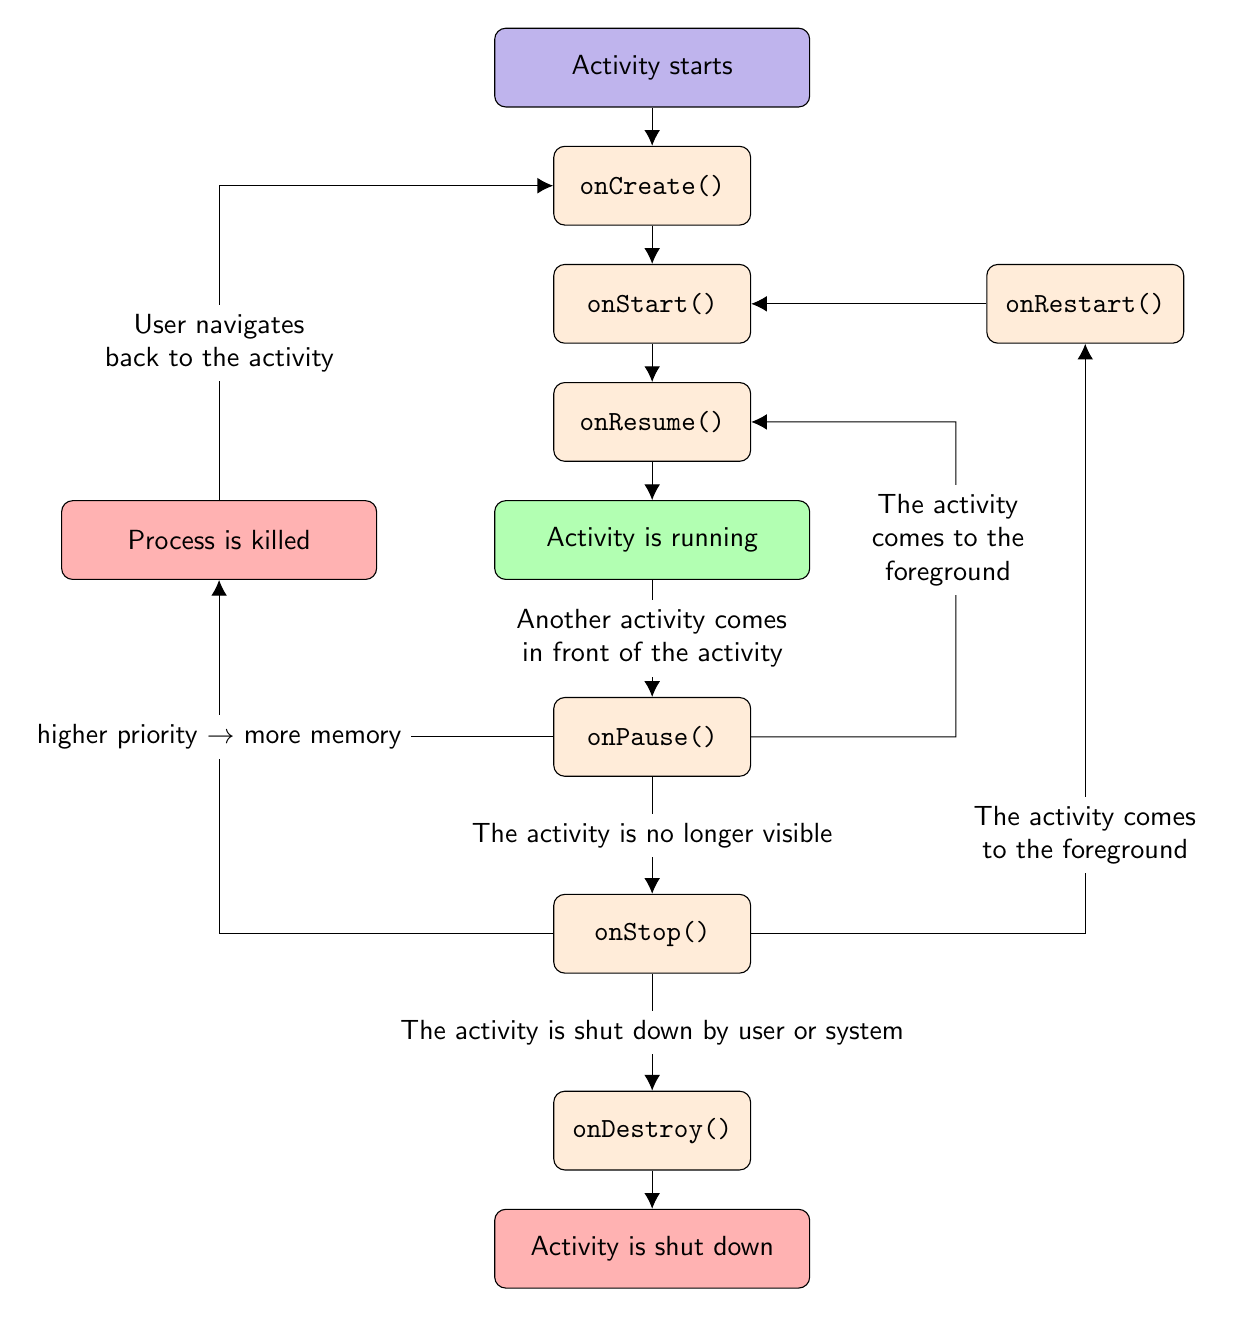
\begin{tikzpicture}[node distance=1.5cm,
every node/.style={fill=white, font=\sffamily}, align=center]
% Specification of nodes (position, etc.)
\node (start)             [activityStarts]              {Activity starts};
\node (onCreateBlock)     [process, below of=start]          {onCreate()};
\node (onStartBlock)      [process, below of=onCreateBlock]   {onStart()};
\node (onResumeBlock)     [process, below of=onStartBlock]   {onResume()};
\node (activityRuns)      [activityRuns, below of=onResumeBlock]
{Activity is running};
\node (onPauseBlock)      [process, below of=activityRuns, yshift=-1cm]
{onPause()};
\node (onStopBlock)       [process, below of=onPauseBlock, yshift=-1cm]
{onStop()};
\node (onDestroyBlock)    [process, below of=onStopBlock, yshift=-1cm] 
{onDestroy()};
\node (onRestartBlock)    [process, right of=onStartBlock, xshift=4cm]
{onRestart()};
\node (ActivityEnds)      [startstop, left of=activityRuns, xshift=-4cm]
{Process is killed};
\node (ActivityDestroyed) [startstop, below of=onDestroyBlock]
{Activity is shut down};     
% Specification of lines between nodes specified above
% with aditional nodes for description 
\draw[->]             (start) -- (onCreateBlock);
\draw[->]     (onCreateBlock) -- (onStartBlock);
\draw[->]      (onStartBlock) -- (onResumeBlock);
\draw[->]     (onResumeBlock) -- (activityRuns);
\draw[->]      (activityRuns) -- node[text width=4cm]
{Another activity comes in
	front of the activity} (onPauseBlock);
\draw[->]      (onPauseBlock) -- node {The activity is no longer visible}
(onStopBlock);
\draw[->]       (onStopBlock) -- node {The activity is shut down by
	user or system} (onDestroyBlock);
\draw[->]    (onRestartBlock) -- (onStartBlock);
\draw[->]       (onStopBlock) -| node[yshift=1.25cm, text width=3cm]
{The activity comes to the foreground}
(onRestartBlock);
\draw[->]    (onDestroyBlock) -- (ActivityDestroyed);
\draw[->]      (onPauseBlock) -| node(priorityXMemory)
{higher priority $\rightarrow$ more memory}
(ActivityEnds);
\draw           (onStopBlock) -| (priorityXMemory);
\draw[->]     (ActivityEnds)  |- node [yshift=-2cm, text width=3.1cm]
{User navigates back to the activity}
(onCreateBlock);
\draw[->] (onPauseBlock.east) -- ++(2.6,0) -- ++(0,2) -- ++(0,2) --                
node[xshift=1.2cm,yshift=-1.5cm, text width=2.5cm]
{The activity comes to the foreground}(onResumeBlock.east);
\end{tikzpicture}
O \textit{framework} tem como objetivo detectar ataques DDoS em tempo real no computador alvo a partir de dados de tráfego de rede com uma taxa aceitável de erros. Tal arcabouço possui três componentes: pré-processamento, um módulo de detecção e um gerente de segurança. Amostras de tráfego são capturadas de uma porta do roteador na forma de um pacote TCP/IP e enviadas ao módulo de pré-processamento. Nessa fase, a cada segundo, os pacotes recebidos são agrupados e essa instância de tráfego é enviada para o módulo de detecção de ataque, que irá classificar a instância como normal ou ataque. O gerente de segurança manterá um perfil normal e um valor limiar em sua base de perfis, para ser usado pelo módulo de detecção. Incrementalmente, o gerente recalcula o perfil normal baseado nos valores anteriores. O último módulo, que é o módulo de segurança irá operar offline e fará análises detalhadas dos \textit{logs} de detecção usando técnicas simplificadas de \textit{machine learning} e estatística. Os componentes citados acima são mais detalhados a seguir.
\subsection{Pré-Processamento}
Nessa etapa, os dados são coletados da rede e, a cada segundo, as métricas desejadas são calculadas para servirem de entrada para a correlação NaHiD. 
\subsubsection{Entropia de IPs origem}
A entropia de IPs origem é uma medida do grau de desordem onde ela é máxima, caso todos os elementos sejam diferentes e o tamanho da entrada é máxima e será mínima (igual a 0) quando todos os elementos são iguais. Assim, a entropia é dada pela seguinte fórmula:
\begin{equation}
H(X) = - \sum_{i}^{n}p(x_i)log_2(x_i)
\end{equation}
Onde $X$ é a entrada e representa os IPs origem das requisições e $n$ é o número total de valores possíveis para o IP origem.  
\subsubsection{Variação de IPs Origem}
Essa medida, diferentemente da entropia, trata-se da taxa de mudança dos IPs origem e é calculada da seguinte forma:
\begin{equation}
	V_{Ip}(X) = \frac{\delta}{N}
\end{equation}
Onde $\delta$ é o número de mudanças de IPs origem e $N$ é o numero total de IPs de entrada. Neste trabalho consideramos uma variação cada troca de valores como no exemplo:
\begin{equation}
	X = {1,2,1,2,3}
\end{equation}
Assim, nesse vetor consideram-se 4 variações ainda que sejam para um valor que repetiu-se. Assim se os IPs origem mudarem frequentemente, a variação será alta. \cite{HOQUE201748}
\\
A observação do comportamento de ataques por \textit{flood} mostra que esse tipo de ameaça pode ser gerada por atacantes reais como zumbis. Se endereços de IP origem falsificados forem utilizados durante um ataque DDoS TCP SYN, a entropia e variação de IPs origem serão altas e esse comportamento também ocorre em um tráfego normal. \cite{HOQUE201748}. Assim faz-se necessário o uso da taxa de pacotes em bits como terceiro medida de entrada para o cálculo da correlação NaHiD.

\subsection{Módulo de Detecção}
O modulo de detecção consiste no uso da correlação NaHiD utilizando os três parâmetros de entrada:
\begin{itemize}
	\item Variação de IPs origem
	\item Entropia de IPs origem
	\item Taxa de pacotes
\end{itemize}
Onde um tráfego normal deve ser fixado para a comparação com o tráfego a ser analisado. Além disso,define-se um limiar do resultado da correlação para distinguir pacotes normais de maliciosos 
\subsection{Gerenciador Offline}
Nessa etapa, os \textit{logs} são salvos e se o módulo de detecção identificar que o tráfego em questão é normal, este será atualizado com os valores do mesmo para a próxima análise

\section{Detecção de Ataques DDoS usando NaHiD}
\label{Sec:NaHiD_VERC}
Para a avaliação do trabalho, duas bases de tráfegos de rede foram escolhidas: DARPA e  DataMining[escolher melhor esse nome] os quais são mais detalhados a seguir 
\subsection{DARPA - MIT}
 A base de dados DARPA foi produzida por pesquisadores do \textit{Lincoln Laboratory} do Instituto de Tecnologia de Massachusetts nos Estados Unidos e tem por objetivo coletar dados de tráfego de rede da Força Aérea do país para encontrar vulnerabilidades em seu sistema bem como ser utilizado para avaliações futuras. Os dados foram coletados e passaram por uma fase de treinamento de 7 semanas com 38 tipos de ataques para simular ameaças internas a rede. O ambiente de rede era composto por duas partes: a rede interna da Força aérea e a rede externa que representava a Internet; ambos conectados por meio de um roteador como mostra a \figref{fig:DARPA_Estrututra}
 \begin{figure}[!htb]
	\caption{Estrutura de rede Base Aérea dos EUA }
	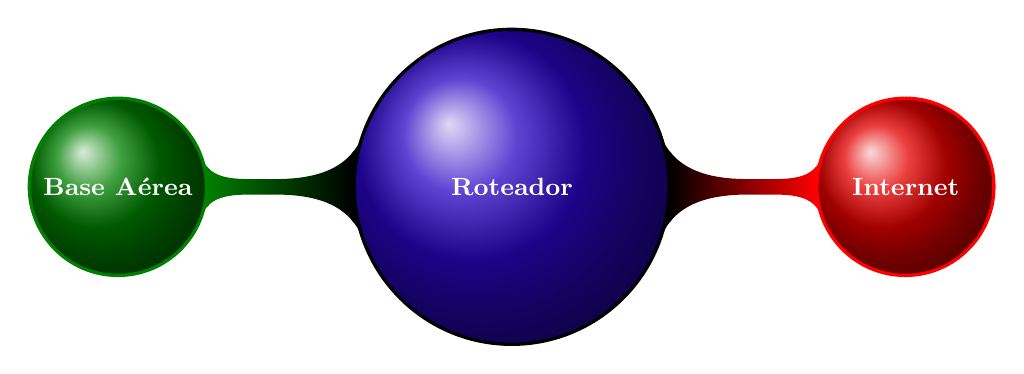
\begin{tikzpicture}
	\path [
	mindmap,
	text = white,
	level 1 concept/.append style =
	{font=\small\bfseries, sibling angle=180},
	level 2 concept/.append style =
	{font=\tiny\bfseries},
	level 3 concept/.append style =
	{font=\tiny\bfseries},
	tex/.style     = {concept, ball color=blue,
		font=\small\bfseries},
	engines/.style = {concept, ball color=green!50!black},
	formats/.style = {concept, ball color=blue!50!black},
	systems/.style = {concept, ball color=red!90!black},
	]
	node [tex] {Roteador} [clockwise from=180]
	child[concept color=green!50!black, nodes={engines}] {
		node {Base Aérea} [clockwise from=90]}
	child [concept color=red, nodes={systems}] {
		node {Internet} [clockwise from=90]};
	\end{tikzpicture}
	{Fonte: Elaborada pelo autor.}
	\label{fig:DARPA_Estrututra}
\end{figure}
\\
Tal banco de dados é disponibilizado pela DARPA em um arquivo de extensão tcpdump, sendo possível extrair informações acerca de cada pacote transmitido durante o período de aquisição dos dados como mostra o exemplo na \tabref{Tab:WiresharkEx}.

\begin{table}[!htb]
	\centering
	\begin{threeparttable}
		\caption{Exemplo base de dados DARPA}
		\label{Tab:WiresharkEx}
		%	\small
		\begin{tabular}{c c c c c c}
			\toprule
			\textbf{Número} & \textbf{Tempo} & \textbf{Origem} & \textbf{Destino}  & \textbf{Protocolo} & \textbf{Tamanho}[bytes]
			\\ \midrule
			1 &  18:56:12.1386 &  192.168.0.20 & 192.168.0.30 & TCP & 60  \\ \midrule
			2 &  18:56:12.1391 & 192.168.0.30 & 192.168.0.20 & TCP & 60  \\ \midrule
			3 &  18:56:12.1588 & 192.168.0.30 & 192.168.0.20 & TELNET & 84  \\ \midrule
			4 &  18:56:12.2099 &  192.168.0.20 & 192.168.0.30 & TCP & 60  \\ \midrule
			5 &  18:56:13.0567 &  192.168.0.20 & 192.168.0.30 & TELNET & 69    \\ \midrule
			6 &  18:56:13.0584 & 192.168.0.30 & 192.168.0.20 & TELNET & 66   \\ \midrule
			7 &  18:56:13.0626 &  192.168.0.20 & 192.168.0.30 & TELNET & 72  \\ \midrule
			8 & 18:56:13.0821 & 192.168.0.30 & 192.168.0.20 & TCP & 60  \\ \bottomrule
		\end{tabular}
		{Fonte: Elaborada pelo autor, baseada em \cite{DARPA}.}
	\end{threeparttable}
\end{table}

No presente trabalho ferramentas como edicap e tcpdump foram utilizadas para o tratamento desse \textit{dataset}. Assim, algumas considerações devem ser feitas:
\begin{itemize}
	\item Janela de um segundo de tráfego
	\item Cálculo de entropia, variação de IPs origem e taxa de pacotes média
	\item Cálculo da correlação NaHiD
\end{itemize}
.
\subsection{DataMining}
Outra base de dados estudada no trabalho foi a desenvolvida por \cite{DataMining} a qual consta em sua totalidade por ataques DDoS de quatro tipos:
\begin{itemize}
	\item SIDDoS
	\item HTTP Flood
	\item UDDP Flood
	\item Smurf
\end{itemize}

A \tabref{Tab:DataMining} mostra os campos do \textit{dataset} 

\begin{table}[!b]
	\centering
	\begin{threeparttable}
		\caption{Estrutura base de dados \cite{DataMining}}
		\label{Tab:DataMining}
		%	\small
		\begin{tabular}{c c }
			\toprule
			\textbf{Número} & \textbf{Tempo}
			\\ \midrule
			1 &  Endereço IP origem  \\ \midrule
			2 &  Endereço IP destino  \\ \midrule
			3 &  Id do pacote  \\ \midrule
			4 &  Nó origem  \\ \midrule
			5 &  Nó destino  \\ \midrule
			6 &  Tipo de pacote  \\ \midrule
			7 &  Tamanho do pacote  \\ \midrule
			8 &  Flags  \\ \midrule
			9 &   Id da flag  \\ \midrule
			10 &  Número de sequência  \\ \midrule
			11 &  Número de pacotes  \\ \midrule
			12 &  Número de bytes  \\ \midrule
			13 &  Nome do nó origem  \\ \midrule
			14 &  Nome do nó destino  \\ \midrule
			15 &  Entrada de pacote  \\ \midrule
			16 &  Saída de pacote  \\ \midrule
			17 &  Taxa de pacotes Recebidos \\ \midrule%%%%%%%%%%%%%%%%%%
			18 &  Atraso de nó do pacote  \\ \midrule
			19 &  Taxa de pacotes\\ \midrule
			20 &  Taxa de bytes  \\ \midrule
			21 &  Tamanho  médio do pacote  \\ \midrule
			22 &  Utilização  \\ \midrule
			23 &  Atraso de pacote  \\ \midrule
			24 &  Tempo de envio do pacote  \\ \midrule
			25 &  Tempo de pacote reservado  \\ \midrule
			26 &  Primeiro pacote enviado  \\ \midrule
			27 &  Último pacote reservado \\ \bottomrule
		\end{tabular}
		{Fonte: Elaborada pelo autor, baseada em \cite{DataMining}.}
	\end{threeparttable}
\end{table}

Algumas considerações foram tomadas para a análise dessa base de dados:
\begin{itemize}
	\item Para construir a janela de um segundo, considerou-se a soma de todos os atrasos por pacote:
	\begin{itemize}
	 \item Atraso de nó do pacote.
	 \item  Atraso de pacote.
	 \item Tempo de pacote reservado.
	\end{itemize}
	\item A média das taxas dos pacotes foi considerada dentro da janela de um segundo.
	\item Por ser um dataset composto apenas por ataques, a comparação com o limiar inverte-se para denotar o quanto dois pacotes são parecidos na correlação.
\end{itemize}

A base de dados é disponibilizada no formato \textit{Weka Attribute-relation}(extensão arff), o qual é utilizado geralmente para compactar grandes massas de dados e processá-las utilizando técnicas de \textit{machine learning}. Assim, para o processamento dos mesmos as ferramentas Weka e MATLAB foram utilizadas.

\externaldocument{algoritmoscomparados}

\chapter[Análise dos Resultados]{Análise dos Resultados}
\label{resultados}
% ----------------------------------------------------------
Neste capítulo, iremos analisar o desempenho dos algoritmos descritos no capítulo anterior. A comparação e determinação de qual algoritmo possui o melhor desempenho será feita utilizando a métrica de satisfação do usuário (a qual foi definida na seção \ref{Satisfacao}). Inicialmente, iremos apresentar os parâmetros utilizados na simulação e posteriormente mostraremos os resultados e discussão destes resultados.

\section{Parâmetros da simulação}

\subsection{Parâmetros gerais}

O ambiente de simulação utilizado neste trabalho leva em consideração as principais características dos sistemas celulares 4G baseados em OFDMA. No capítulo \ref{Simulacao}, descrevemos as características do nosso simulador. Na tabela \ref{Tab:Gen_Simul_Param} são mostrados os parâmetros gerais de simulação utilizados.

\renewcommand{\arraystretch}{1}
\begin{table}[!ht]
	\centering
	\begin{threeparttable}[t]
		\caption{Parâmetros gerais da simulação.}
		\label{Tab:Gen_Simul_Param}
		\centering
		\tiny
		\begin{tabular}{l l}
			\toprule
			\textbf{Parâmetro} & \textbf{Valor}\\
			\midrule
			Potência máxima de transmissão da BS\tnote{a} & 12 W \cite{3gpp.36.814}\\
			\midrule
			Setorização da antena da BS & 3 setores de 120$^{\circ}$ \cite{3gpp.36.814}\\
			\midrule
			Raio da célula & 1 km\\
			\midrule
			Velocidade dos dispositivos móveis & 3 km/h \cite{3gpp.25.814}\\
			\midrule
			Largura de banda do sistema & 3 MHz \cite{Book:Pelcat2013}\\
			\midrule
			Quantidade de RBs & 15 \cite{Book:Pelcat2013}\\
			\midrule
			Tempo de coerência do canal & 90 ms\\
			\midrule
			Ganho da antena\tnote{b} & $G_{h}(\theta_{h}) + G_{v}(\theta_{v}$) \cite{Gunnarsson2008}\\
			\midrule
			Ângulo de \textit{Downtilt} & 8$^{\circ}$\\
			\midrule
			Desvio padrão do sombreamento lognormal ($\sigma_{\mathrm{sh}}$) & 8 dB \cite{3gpp.25.814}\\
			\midrule
			Desvanecimento de pequena escala & 3GPP \textit{Typical Urban} \cite{3gpp.25.943}\\
			\midrule
			Potência AWGN por subportadora & -123.24 dBm\\
			\midrule
			Figura de ruído & 9 dB\\
			\midrule
			Limite de SNR da MCS 1 & -6.9 dB \cite{EUSIPCO2009}\\
			\midrule
			Degradação da CSI ($\psi$) & 0,05\\
			\midrule
			Atraso da CSI ($\Delta n$) & 15 TTIs\\
			\midrule
			Tempo da sessão de simulação & 30 segundos\\
			\midrule
			Número de simulação executadas & 90 \\
			\bottomrule
		\end{tabular}
		\begin{tablenotes}
			\item [a] Valor utilizado devido à quantidade de RBs utilizadas.
			\item [b] $\theta_{h}$ e $\theta_{v}$ representam os ângulos horizontal e vertical relacionados com a BS, respectivamente.
		\end{tablenotes}
		{Fonte: Elaborada pelo autor.}
	\end{threeparttable}
\end{table}

\subsection{Parâmetros dos modelos de tráfego}

A descrição dos modelos de tráfego utilizados para compor o cenário com múltiplos serviços foi apresentada no capítulo \ref{Simulacao}. No entanto, o valor dos parâmetros utilizados para os modelos de tráfego ainda não foram especificados. Na tabela \ref{Tab:Par_VOIP} mostramos os parâmetros utilizados para o tráfego VoIP e na tabela \ref{Tab:Par_CBR} mostramos os parâmetros utilizados para o tráfego CBR. 

\begin{table}[!ht]
	\centering
	\begin{threeparttable}[t]
		\caption{Parâmetros do modelo de tráfego VoIP.}
		\label{Tab:Par_VOIP}
		\centering
		\small
		\begin{tabular}[t]{ll}
			\toprule
			\textbf{Parâmetro} & \textbf{Valor}\\
			\midrule
			Tamanho do pacote & 320 bits\\
			\midrule
			Intervalo entre chegada de pacotes & 20 ms\\
			\midrule
			Duração da chamada & 30 segundos\\
			\midrule
			Média de tempo dos estados da cadeia de Markov & 1 s\\
			\midrule
			Fator de atividade & 50\%\\
			\midrule
			Limite para a FER ($\text{FER}_{\text{req}}^{\text{rt}}$)& 2\%\\
			\midrule
			Limite de tempo do pacote HOL($\Phi_{\text{req}}^{\text{rt}}$) & 20 ms\\
			\bottomrule
		\end{tabular}
		{Fonte: Elaborada pelo autor.}
	\end{threeparttable}
\end{table}

\begin{table}[!ht]
	\centering
	\begin{threeparttable}[t]
		\caption{Parâmetros do modelo de tráfego CBR.}
		\label{Tab:Par_CBR}
		\centering
		\small
		\begin{tabular}[t]{ll}
			\toprule
			\textbf{Parâmetro} & \textbf{Valor}\\
			\midrule
			Taxa de geração de pacotes & 512~kbps\\
			\midrule
			Tamanho do pacote & 2048 bits\\
			\midrule
			Intervalo entre chegada de pacotes & 4 ms\\
			\midrule
			Duração da sessão & 30 segundos\\
			\midrule
			Média de tempo dos estados da cadeia de Markov & 1 s\\
			\midrule
			Fator de atividade & 50\%\\
			\midrule
			Limite de tempo do Pacote HOL & 200 ms\\
			\midrule
			Requerimento de vazão de dados ($\Phi_{\text{req}}^{\text{nrt}}$) & 512~kbps \\
			\bottomrule
		\end{tabular}
		{Fonte: Elaborada pelo autor.}
	\end{threeparttable}	
\end{table}

\subsection{Parâmetros dos algoritmos estudados}

Como os modelos de tráfego utilizados neste trabalho são diferentes em relação aos valores dos parâmetros dos modelos analisados em \citeonline{Phd:Song2005}, \citeonline{Proc:Lei2007}, \citeonline{Nasralla2013} e \citeonline{basukala2009performance}, algumas adaptações foram feitas para que os algoritmos de comparação tivessem suas propostas mantidas. Vale ressaltar que as adaptações foram feitas considerando as propostas iniciais dos autores e as magnitudes relativas das prioridades atribuídas originalmente para cada classe de serviço fossem mantidas.    

Como o algoritmo EXP/PF não depende dos parâmetros referentes aos modelos de tráfego, este algoritmo não sofreu nenhuma modificação. Em relação ao algoritmo QHMLWDF, também não há parâmetros que dependem dos tráfegos considerado. Para o QHMLWDF, apenas foi considerado que $\alpha[n] = 0,1$, o que significa que a máxima probabilidade aceitável que os pacotes excedam o tempo limite é 10\% da quantidade total de pacotes enviados. 

Os algoritmos MDU e \textit{Utility} Lei possuem parâmetros que são definidos de acordo com os modelos de tráfego considerados. Para o algoritmo MDU, existem 3 possíveis funções de utilidade que podem ser consideradas. Como neste trabalho utilizamos o serviço VoIP e o serviço CBR, iremos utilizar as funções de utilidade referentes ao VoIP e \textit{Streaming} (uma vez que o serviço CBR pode ser considerado um tipo de \textit{streaming} com taxa constante) que foram propostas em \citeonline{Phd:Song2005}. No entanto, como os valores dos parâmetros dos modelos de tráfego são um pouco diferentes, as funções para o serviço VoIP ($ |U^{'}_V(\text{w})|$) e o serviço CBR ($|U^{'}_S(\text{w})|$) ficam:
%
\begin{equation}
\label{Eq:VoIPAlt}
\left| U^{'}_V(\text{w}) \right| = \begin{cases} 
\text{w}[n]^{2,9}, & \text{if  } \text{w}[n] \leq \text{5 ms} \\ 
\text{w}[n]^{2,9} - 5^{2,9} + 5, & \text{if  } \text{w}[n] >  \text{5 ms}; 
\end{cases}
\end{equation} 
%
\begin{equation}
\label{Eq:StreamingAtl}
\left| U^{'}_S(\text{w}) \right| = \begin{cases} 
\text{w}[n], & \text{if  } \text{w}[n] \leq \text{50 ms} \\ 
\text{w}[n]^{1,5} - 50 + 50^{1,5}, & \text{if  } \text{w}[n] >  \text{50 ms},
\end{cases}
\end{equation}
%
em que os 5~ms de $ |U^{'}_V(\text{w})|$ refere-se a 0,25\% $\cdot$ 20~ms (tempo limite do pacote HOL do VoIP) e 50~ms de $|U^{'}_S(\text{w})|$ refere-se a 0,25\% $\cdot$ 200~ms (tempo limite do pacote HOL do CBR), seguindo o que foi proposto originalmente. Dessa forma, a magnitude e prioridade relativa entre esses serviços mostradas na figura \ref{fig:WeightSong} são mantidas.
Para o algoritmo \textit{Utility} Lei, os parâmetros das funções de utilidade foram redefinidos para os seguintes valores: $\beta = 450$, $\Phi_{\text{req}}^{\text{rt}} = 20 \text{ ms}$, $a = 5$, $b = 0,5$ e $c = 200 \text{ ms}$. Com isso a magnitude e prioridade relativa entre os serviços considerados mostradas nas figuras \ref{fig:PrimitiveWeightLEI} e \ref{fig:WeightLEI} são mantidas.

\section{Resultados e discussão}

Nesta seção iremos mostrar os resultados obtidos para o desempenho dos algoritmos estudados. Como já mencionado, a métrica utilizada para realizar a comparação será a métrica de satisfação do usuário. Primeiramente iremos mostrar os resultados para cenários com serviço único e posteriormente iremos mostrar os resultados para cenários com múltiplos serviços. Todos os resultados das simulações neste trabalho são apresentados com 95\% de intervalo de confiança da média das amostras, os quais serão ilustrados como barras verticais ou horizontais em torno de um determinado ponto.  

A definição de qual algoritmo possui melhor desempenho será feita analisando o Plano de Capacidade Conjunta do sistema, que é uma ferramenta poderosa para análise de resultados, já que ela fornece uma forma completa de avaliação condensando os resultados para cenários com serviço único e múltiplos serviços em um único gráfico.

As figuras apresentadas nesta seção ilustrarão gráficos onde o eixo das abscissas é o número de usuários por célula e o eixo das ordenadas é a porcentagem de usuários satisfeitos em cada célula. Este será o modelo de apresentação dos resultados seguido neste trabalho. Além disso, pode-se perceber que existe uma linha horizontal para o nível de satisfação de 90\%, a qual será entendida e utilizada quando estivermos explicando e definindo o Plano de Capacidade Conjunta.

\subsection{Cenário com serviço único RT}

Nesta seção, mostraremos os resultados obtidos para o cenário composto apenas por usuários utilizando o serviço VoIP, ou seja, apenas usuários de serviço RT.

A figura \ref{fig:VoIPAll} ilustra o gráfico da satisfação dos usuários obtido neste cenário. A quantidade de usuários por célula foi incrementada de 50 usuários inicialmente, e de 10 em 10 usuários após 180 usuários por célula. Perceba que o eixo que indica a porcentagem de usuários satisfeitos varia de 0.4 até 1, já que nenhum algoritmos apresentou desempenho pior que 40\% dos usuários satisfeitos. 

Nota-se que o desempenho dos algoritmos é relativamente parecido até a carga de 240 usuários VoIP. A partir deste ponto, o desempenho do algoritmo \textit{Utility} Lei decresce drasticamente, conseguindo satisfazer apenas aproximadamente 42\% dos usuários para a carga de 300 usuários. A última carga de usuários em que o algoritmo \textit{Uitlity} Lei consegue manter a satisfação acima de 90\% é 240 usuários. Os motivos para que o desempenho do algoritmo \textit{Uitlity} Lei decresça drasticamente com altas cargas de usuários são o formato da função de utilidade utilizada para alocar os recursos para o serviço RT (equação \ref{Eq:LeiMarginalRT}) e a característica oportunística deste algoritmo. 

\begin{figure}[htb]
	\centering	
	
	\caption[Satisfação dos usuários para cenário com apenas usuários VoIP]{Satisfação dos usuários para cenário com apenas usuários VoIP.}
	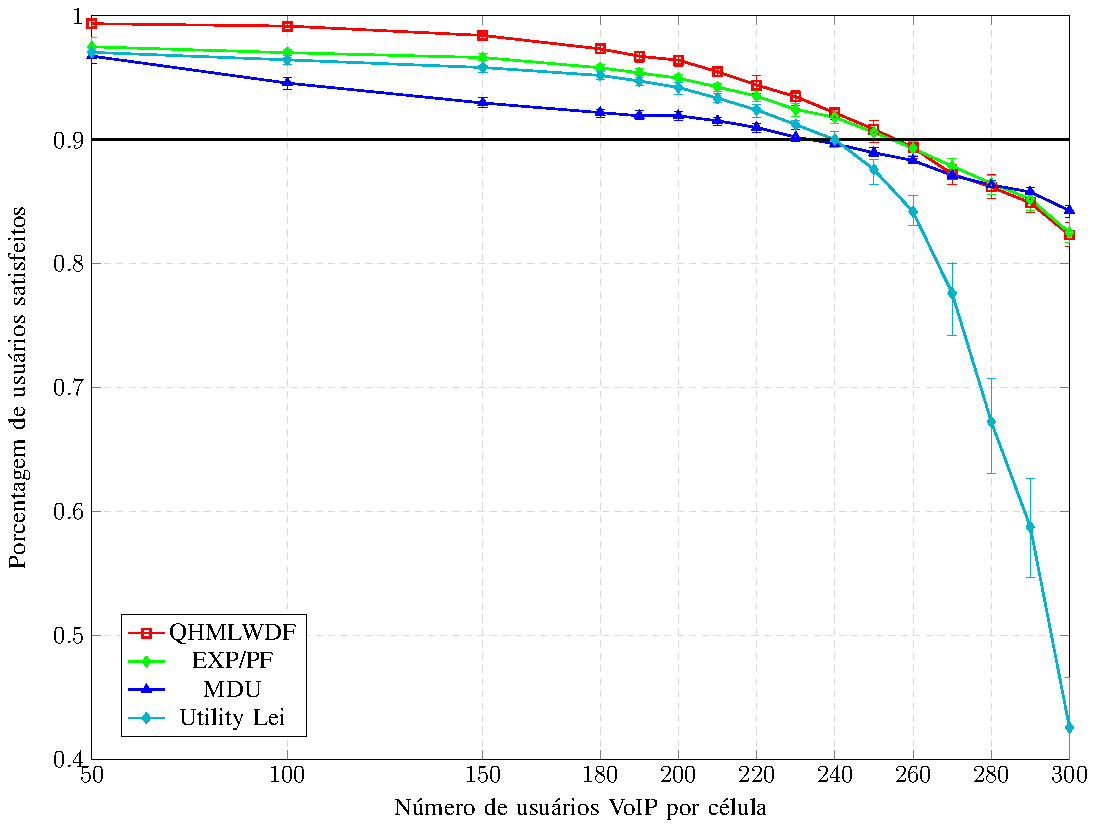
\includegraphics[width=1\textwidth]{figs/VOIPAll.pdf}
	
	{Fonte: Elaborada pelo autor.}
	\label{fig:VoIPAll}
\end{figure}

Os outros três algoritmos estudados conseguem manter a satisfação dos usuários em níveis aceitáveis mesmo após a carga de 240 usuários. Perceba que mesmo com 300 usuários por célula, os algoritmos MDU, EXP/PF e QHMLWDF conseguem uma porcentagem de satisfação acima de 80\%. A última carga com satisfação acima de 90\% para MDU, EXP/PF e QHMLWDF são 240, 260 e 260, respectivamente. O algoritmo EXP/PF consegue atingir esse desempenho devido ao fato de utilizar o atraso do pacote HOL como principal métrica para alocação dos recursos, dando maior prioridade para usuários que estão com atraso maior que a média dos atrasos dos usuários ativos (equação \ref{Eq:EXPPF_RT}), o que faz com que o atraso médio dos usuários seja baixo. O algoritmo MDU alcança esse desempenho utilizando a informação do tamanho da fila dos usuários para fazer a alocação dos recursos (equação \ref{Eq:MDU_RT}), fazendo com que os usuários com maior tamanho da fila tenha maior prioridade e, portanto, mantendo o atraso dos usuários o mais baixo possível. Já o algoritmo QHMLWDF, combina as métricas de atraso do pacote HOL e tamanho da fila de pacotes (equação \ref{Eq:QHMLWDF_RT_NRT}) para manter a PLR dos usuários em baixos níveis,  alcançando bom desempenho neste cenário. 

A conclusão que podemos tirar deste resultado parcial é que as abordagens que utilizam tempo de espera médio (MDU), atraso do pacote HOL (EXP/PF) e tamanho da fila de pacotes e atraso do pacote HOL (QHMLWDF) foram eficazes na tarefa de satisfazer os usuários RT. Apesar do algoritmo \textit{Utility} Lei também utilizar o atraso do pacote HOL como métrica para alocação dos recursos, este algoritmo não obteve resultados tão bons quanto os outros algoritmos, o que pode ser explicado devido ao formato ou inclinação da função de utilidade que foi proposta.

\subsection{Cenário com serviço único NRT}

Nesta seção, mostraremos os resultados obtidos para o cenário composto apenas por usuários utilizando o serviço CBR, ou seja, apenas usuários de um serviço que assumimos como NRT.

A figura \ref{fig:CBRAll} ilustra o gráfico da satisfação dos usuários obtido neste cenário com usuários CBR. A quantidade de usuários por célula foi incrementada de 1 usuário a partir da quantidade inicial de 10 usuários até a carga de 20 usuários. Após isso, a carga de usuários foi incrementada de 2 em 2. Perceba que a granularidade da quantidade de usuários por célula é bem menor para este tipo de serviço. Note também que o eixo que indica a porcentagem de usuários satisfeitos varia de 0.3 até 1, já que nenhum algoritmos apresentou desempenho pior que 30\% dos usuários satisfeitos. 

Pode ser facilmente percebido que o algoritmo EXP/PF apresentou o melhor desempenho neste cenário. O nível de satisfação obtido por este algoritmo ficou acima do nível de satisfação dos outros algoritmos para todas as cargas consideradas. A carga de 26 usuários é a última em que o EXP/PF consegue manter a satisfação acima de 90\%. O principal motivo para isto é que o algoritmo EXPPF utiliza a vazão de dados dos usuários como principal métrica para fazer a alocação dos recursos para o serviço NRT (equação \ref{Eq:EXPPF_NRT}), a qual é a métrica que define a satisfação para esta classe de serviço. Por outro lado, o algoritmo QHMLWDF foi o que obteve pior desempenho. Para a carga máxima analisada de 28 usuários, este algoritmos atingiu menos de 30\% de satisfação, que foi a mais baixa entre os algoritmos analisados. A última carga com satisfação acima de 90\% para o QHMLWDF foi de 14 usuários. Isso ocorreu pelo fato de que este algoritmo foi proposto para manter a PLR dos usuários em baixos níveis por meio do uso das métricas de atraso e tamanho da fila, mas manter a PLR em baixos níveis não garante que usuários NRT estejam satisfeitos. 

Os outros dois algoritmos, a saber MDU e \textit{Utility} Lei, obtiveram resultados medianos neste cenário. Apesar de a última carga em que a satisfação ficou acima de 90\% para o MDU, que foi de 15 usuários CBR, ter sido bem parecida com a do pior algoritmo, o MDU conseguiu sustentar a satisfação dos usuários em níveis mais altos a medida que a carga de usuários foi aumentando. Para o \textit{Utility} Lei, a última carga com satisfação de acima de 90\% foi de 19 usuários CBR.

Uma conclusão parcial obtida depois da observação dos resultados para o cenário com apenas o serviço NRT foi: a melhor abordagem foi a do EXP/PF, que aloca os recursos para os usuários CBR com base no valor da vazão de dados destes usuários, atacando diretamente a métrica que define a satisfação deste tipo de serviço. A abordagem que utiliza tamanho da fila de pacotes e atraso do pacote HOL do QHMLWDF não se mostrou eficaz para este cenário.

\begin{figure}[htb]
	\centering	
	
	\caption[Satisfação dos usuários para cenário com apenas usuários CBR]{Satisfação dos usuários para cenário com apenas usuários CBR.}
	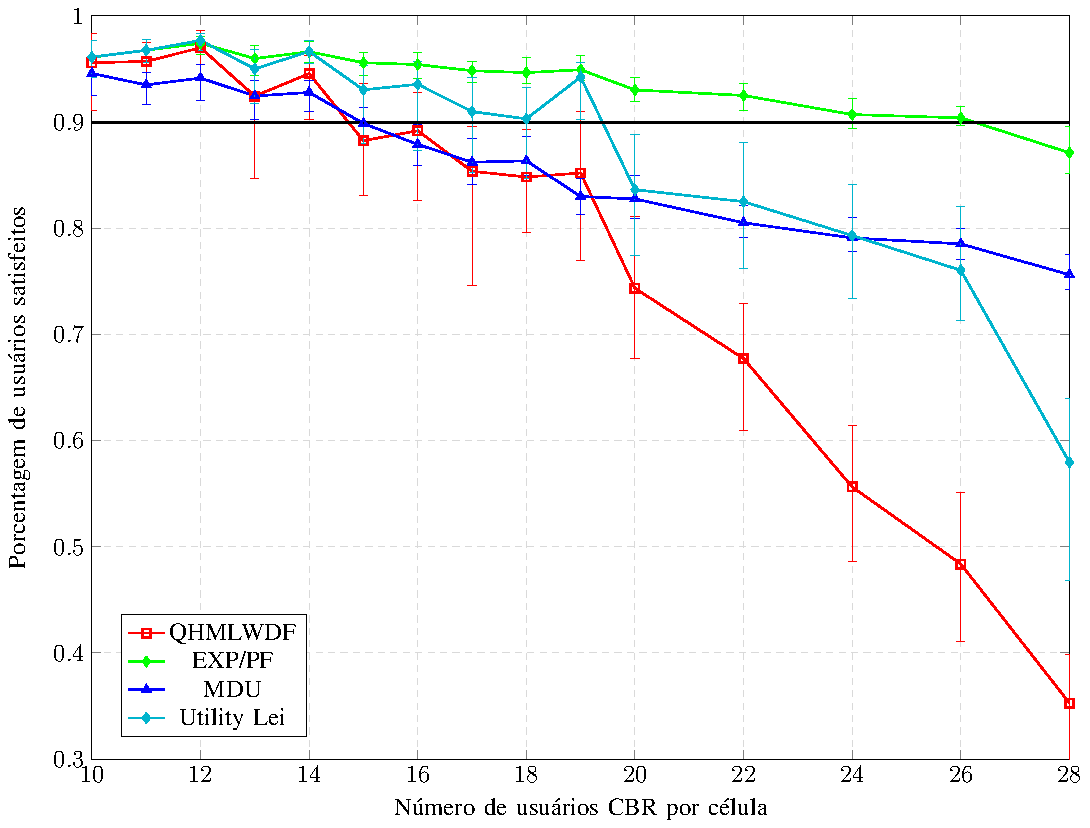
\includegraphics[width=1\textwidth]{figs/CBRAll.pdf}
	
	{Fonte: Elaborada pelo autor.}
	\label{fig:CBRAll}
\end{figure}

\subsection{Cenário com múltiplos serviços}

A partir de agora, iremos mostrar os resultados para cenários compostos por uma mistura de usuários utilizando serviços NRT (CBR) e RT (VoIP). Nos gráficos que ilustram os resultados para este cenário, o eixo das abscissas apresenta a quantidade total de usuários presentes na célula, ou seja, é uma soma da quantidade de usuários CBR e de usuários VoIP. 

A abordagem utilizada para obtenção dos resultados para este cenário foi a seguinte: a quantidade de usuários VoIP era fixada em um determinado número, a saber 100, 150 e 200, e a quantidade de usuários CBR era variada. O critério de parada na variação do número de usuários CBR era o momento em que a satisfação dos dois serviços ficava abaixo de 90\%. Note que o eixo que indica a porcentagem de usuários satisfeitos para este varia de 0 até 1, já que alguns algoritmos apresentaram desempenho bem baixo neste cenário. 

Na figura \ref{fig:100VOIP} mostramos os resultados para o cenário com 100 usuários VoIP e uma quantidade variável de usuários CBR. Pode-se notar que em relação a satisfação do serviço RT, os algoritmos EXP/PF e MDU obtiveram os melhores resultados. Apesar disso, se consideramos a satisfação de uma forma conjunta para os dois serviços, o desempenho do algoritmo EXP/PF foi melhor, o que ocorreu devido ao fato de o EXP/PF utilizar as principais métricas que definem a satisfação de cada tipo serviço, a saber atraso do pacote HOL para o serviço RT e vazão de dados para o serviço NRT. Perceba que os algoritmos EXP/PF e o MDU mantiveram a satisfação do serviço RT sempre acima de 90\%. O MDU consegue manter a satisfação do serviço RT sempre em altos níveis porque este serviço sempre tem maior prioridade na alocação dos recursos (figura \ref{fig:WeightSong}). Já o algoritmo EXP/PF mantém sempre o nível de satisfação do serviço RT mais alto pelo fato de a magnitude da fórmula que define a prioridade do serviço RT (equação \ref{Eq:EXPPF_RT}) ser maior que a magnitude da fórmula para o serviço NRT (equação \ref{Eq:EXPPF_RT}). 

\begin{figure}[hb]
	\centering
	
	\caption[Satisfação dos usuários para cenários com 100 usuários VoIP e um número variável de usuários CBR]{Satisfação dos usuários para cenários com 100 usuários VoIP e um número variável de usuários CBR.}
	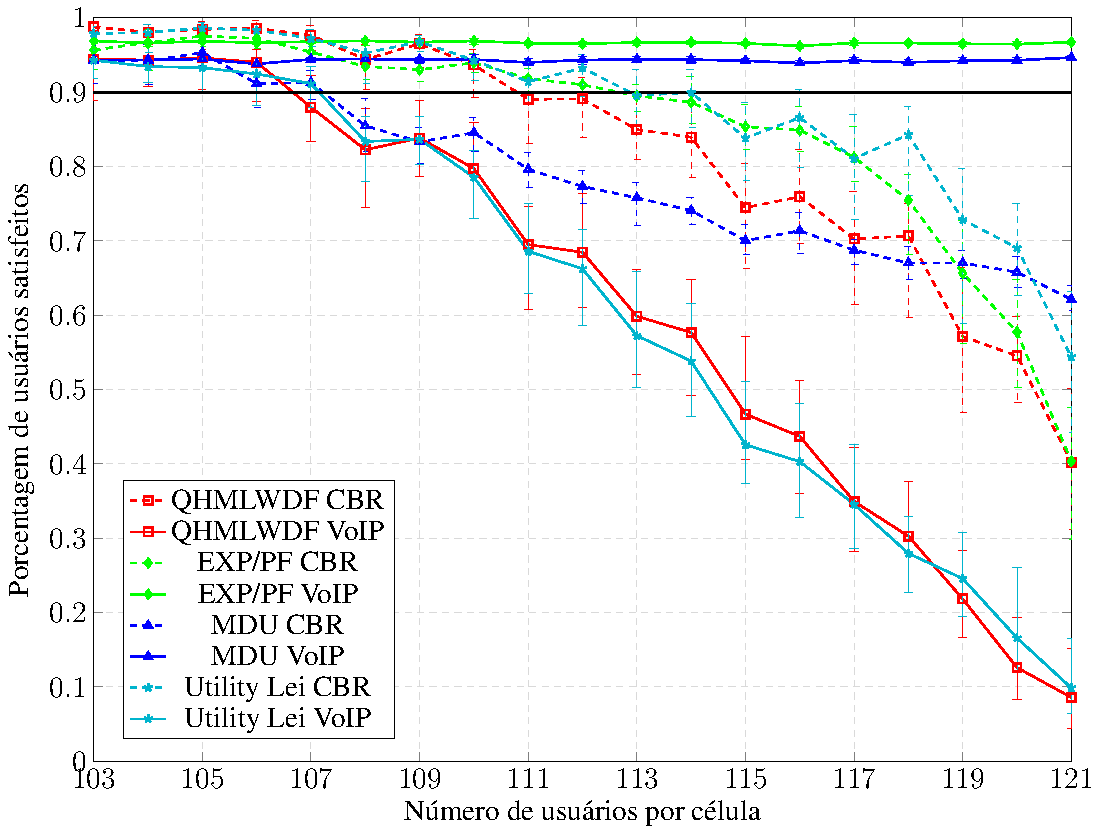
\includegraphics[width=.8\linewidth]{figs/100VOIP.pdf}
	
	{Fonte: Elaborada pelo autor.}
	\label{fig:100VOIP}
\end{figure}

O terceiro melhor desempenho neste cenário foi obtido pelo algoritmo QHMLWDF, enquanto que o algoritmo \textit{Utility} Lei obteve o pior resultado em termos de satisfação conjunta. A última carga de usuários tal que a satisfação ficou acima de 90\% para os dois serviços será mostrada apenas no plano de capacidade conjunta, que será apresentado na próxima subseção. Perceba que para os algoritmos QHMLWDF e \textit{Utility} Lei o nível de satisfação do serviço NRT é sempre mais alto que a satisfação do serviço RT, o que é um comportamento contrário ao apresentado pelos algoritmos EXP/PF e MDU. Para o algoritmo QHMLWDF, isso ocorre pelo fato que este algoritmo utilizar o tamanho da fila para fazer a alocação dos recursos. Como a taxa de geração de pacotes do serviço CBR (512~Kbps, olhar tabela \ref{Tab:Par_CBR}) é maior que a taxa de geração de pacotes do serviço VoIP (16~Kbps, olhar tabela \ref{Tab:Par_VOIP}), o tamanho da fila dos usuários CBR é normalmente maior que a fila dos usuários VOIP, fazendo com que os usuários CBR tenham maior prioridade. Para o algoritmo \textit{Utility} Lei, a satisfação dos usuários NRT é maior que a satisfação dos usuários RT devido ao formato das curvas que definem as prioridades de cada serviço (olhar figura \ref{fig:WeightLEI}). Perceba que quando o atraso do pacote HOL está em valores baixo, o serviço RT tem maior prioridade. Para atrasos mais altos, a prioridade do serviço NRT tende a ser maior. Como o limite de tempo do pacote HOL para o serviço CBR é maior que o limite de tempo do pacote HOL para o serviço VoIP (olhar tabelas \ref{Tab:Par_CBR} e \ref{Tab:Par_VOIP}), a prioridade do serviço CBR tende a ser maior que a prioridade do serviço VOIP. 

\begin{figure}[b]
	\centering
	
	\caption[Satisfação dos usuários para cenários com 150 usuários VoIP e um número variável de usuários CBR]{Satisfação dos usuários para cenários com 150 usuários VoIP e um número variável de usuários CBR.}
	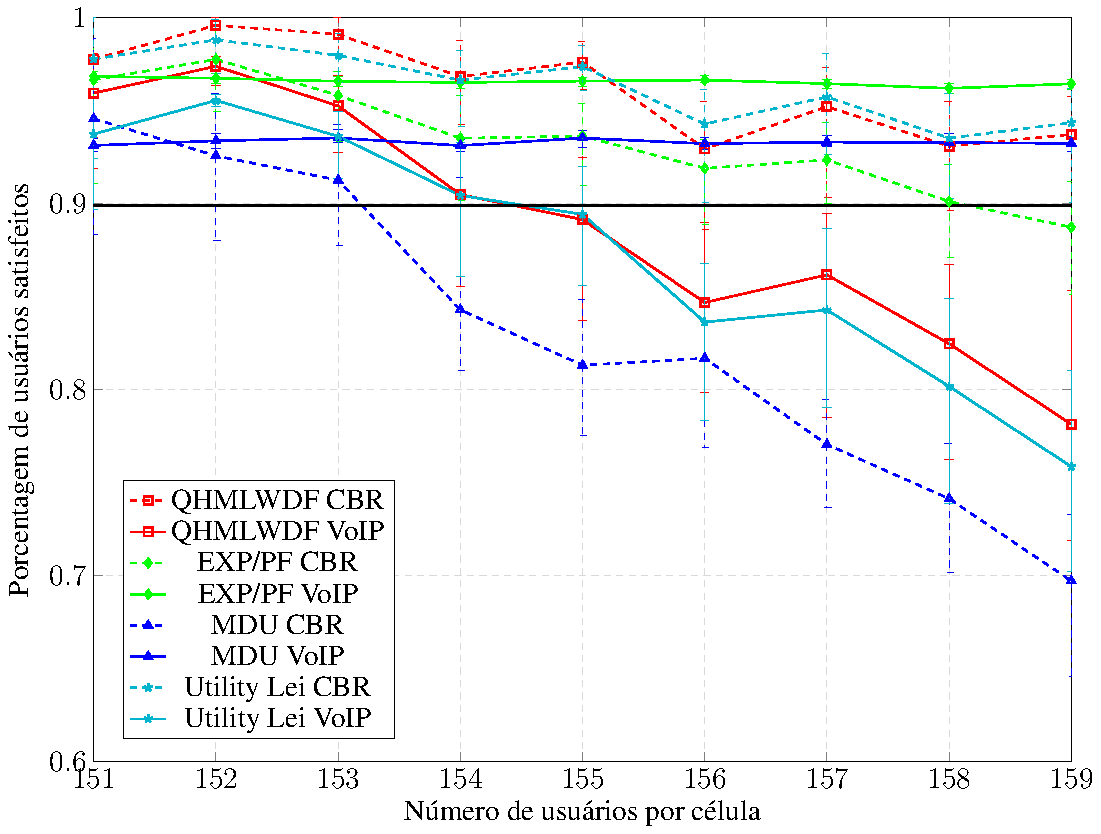
\includegraphics[width=.8\linewidth]{figs/150VOIP.pdf}
	
	{Fonte: Elaborada pelo autor.}	
	\label{fig:150VOIP}
\end{figure}

Na figura \ref{fig:150VOIP} mostramos os resultados para o cenários com 150 usuários VoIP e uma quantidade variável de usuários CBR. Perceba que a medida que vamos aumentando a quantidade fixa de usuários VoIP, a quantidade de usuários CBR suportados vai obviamente diminuindo. Note que o eixo que indica a porcentagem de usuários satisfeitos varia de 0.6 até 1, já que nenhum algoritmos apresentou desempenho pior que 60\% dos usuários satisfeitos. 

Pode-se notar que, em relação a satisfação conjunta, o algoritmo EXP/PF novamente obteve o melhor resultado (o motivo para isso já foi explicado anteriormente). O algoritmo MDU  obteve o pior desempenho para esta quantidade de usuários VoIP. Isso ocorreu porque a prioridade do serviço RT é absolutamente maior que a prioridade do serviço NRT, o que fez com que os usuários CBR não recebessem recursos. Os outros dois algoritmos, QHMLWDF e \textit{Utility} Lei, obtiveram desempenhos similares para este cenários, tanto em relação à satisfação dos usuários CBR quanto em relação à satisfação do serviço RT.

Na figura \ref{fig:200VOIP} mostramos os resultados para o cenários com 200 usuários VoIP e uma quantidade variável de usuários CBR. Para esta quantidade de usuários VoIP, foi necessário apenas que realizássemos simulações com até 5 usuários CBR. Perceba que o eixo que indica a porcentagem de usuários satisfeitos varia de 0.5 até 1.

Note que para este cenário específico, o desempenho de todos os algoritmos, com exceção do algoritmo MDU, foram consideravelmente próximos. O motivo de o desempenho do algoritmo MDU ter sido o pior foi explicado no parágrafo anterior. A última carga suportada com satisfação acima de 90\% obtida pelos algoritmos EXP/PF, QHMLWDF e \textit{Utility} Lei foi de 202 usuários, ou seja, 200 usuários VoIP mais 2 usuários CBR, o que nos leva a concluir que este é o limite máximo de satisfação que pode ser obtido neste cenário, considerando os algoritmos analisados neste estudo. O algoritmo MDU conseguiu apenas manter a satisfação dos usuários VoIP acima de 90\% para este cenário.

Uma forma de condensar os resultados ilustrados nas figuras \ref{fig:VoIPAll}, \ref{fig:CBRAll}, \ref{fig:100VOIP}, \ref{fig:150VOIP}, \ref{fig:200VOIP} em um único gráfico é através do plano de capacidade conjunta, que será definido a partir de agora.

\begin{figure}
	\centering
	
	\caption[Satisfação dos usuários para cenários com 200 usuários VoIP e um número variável de usuários CBR]{Satisfação dos usuários para cenários com 200 usuários VoIP e um número variável de usuários CBR.}
	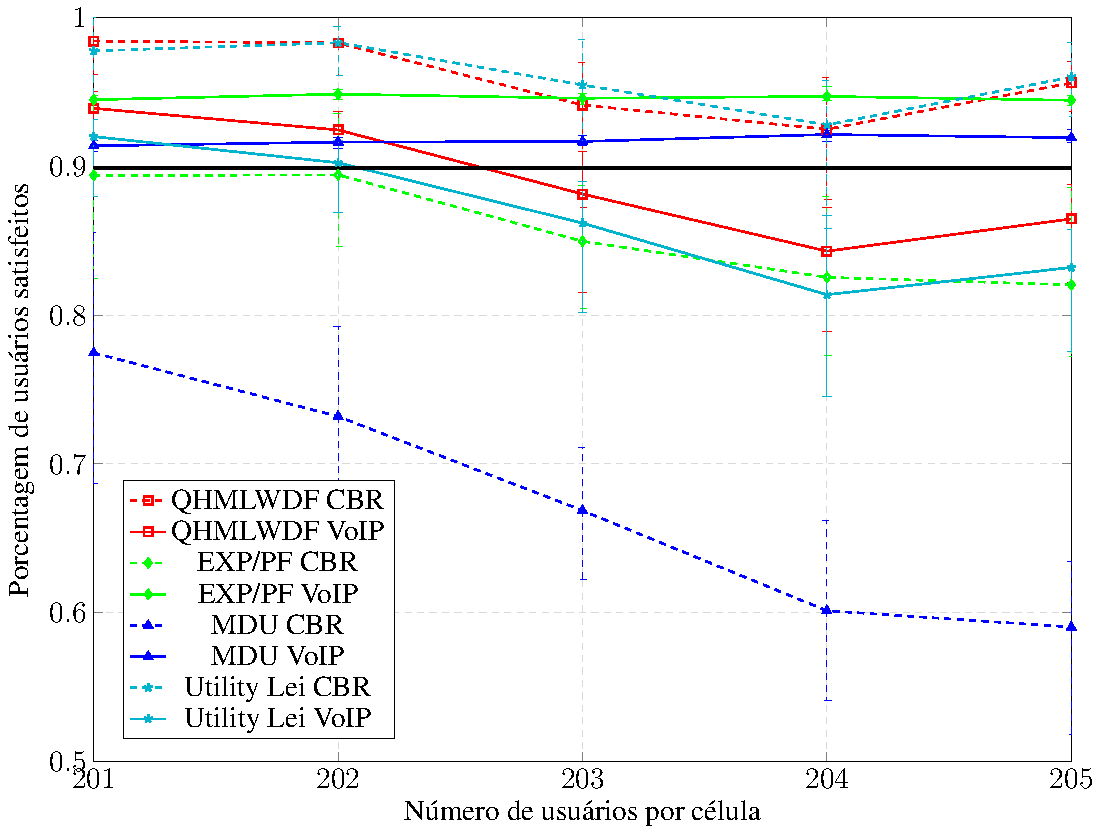
\includegraphics[width=.8\linewidth]{figs/200VOIP.pdf}
	
	{Fonte: Elaborada pelo autor.}
	\label{fig:200VOIP}
\end{figure}

\subsubsection{Plano de capacidade conjunta}

Como já mencionado, o plano de capacidade conjunta é uma ferramenta poderosa para analisar o desempenho de algoritmos de RRA em cenários com múltiplos serviços. Este plano mostra as regiões de capacidade do sistema que podem ser definidas como o número de usuários para o qual os níveis de QoS são mantidos acima de um determinado limiar para todas as classes de serviço ao mesmo tempo.

Considerando os cenários com apenas um tipo de serviço, o ponto de interesse para a construção do plano de capacidade conjunta é aquela carga (número de usuários) tal que os algoritmos são capazes de manter a porcentagem de usuários satisfeitos acima de um determinado nível. 
% Verificar se isto foi dito antes?
Neste trabalho, este nível é 90\% de usuários satisfeitos. Este é o motivo pelo qual uma linha horizontal foi traçada neste nível de satisfação nas figuras \ref{fig:VoIPAll}, \ref{fig:CBRAll}, \ref{fig:100VOIP}, \ref{fig:150VOIP}, \ref{fig:200VOIP}. O valor desta carga dos cenários com um único serviço são utilizadas para achar os pontos que compõem o eixo das abscissas e das ordenadas no plano de capacidade conjunta.

Em relação aos cenários com múltiplos serviços, o valor da capacidade conjunta do sistema é definida como a capacidade máxima que os algoritmos de RRA suportam para ambos os serviços tal que uma determinada qualidade seja garantida para ambos os serviços de forma simultânea. Esta determinada qualidade é definida neste trabalho como nível de QoS e refletida na porcentagem de usuários satisfeitos, que deve estar acima de 90\% para os dois serviços ao mesmo tempo. Os pontos obtidos seguindo este critério são utilizados para construir os pontos do interior do plano de capacidade conjunta.

Na figura \ref{fig:CapPlane} está ilustrado o plano de capacidade conjunta que foi obtido seguindo os critérios definidos nos dois parágrafos anteriores. O desempenho de cada algoritmo de RRA estudado neste trabalho é ilustrado como uma curva de capacidade neste gráfico. Os pontos obtidos a partir das figuras  \ref{fig:VoIPAll} e \ref{fig:CBRAll} foram utilizados para plotar os pontos das ordenadas e abscissas, respectivamente. As cargas que foram extraídas das figuras \ref{fig:100VOIP}, \ref{fig:150VOIP}, \ref{fig:200VOIP} foram utilizados para completar as curvas de capacidade de cada algoritmo de RRA, ligando os pontos extremos das abscissas e coordenadas. Perceba que o intervalo de confiança para este gráfico é representado como intervalos na horizontal em torno de um ponto, representando um variabilidade na quantidade de usuários CBR suportados para uma certa carga de usuários VoIP.

Quanto maior for a área abaixo do gráfico, maior é a porcentagem de usuários satisfeitos respeitando um limite de satisfação mínimo de 90\%. Portanto, pode-se notar que o algoritmo que obteve o melhor desempenho entre todos foi o EXP/PF. Este algoritmo obteve o melhor desempenho para o cenário com serviço único NRT (eixo das abscissas) e também obteve o melhor desempenho para o cenário com serviço único RT (eixo da ordenadas), onde empatou com o algoritmo QHMLWDF. Considerando o cenário com 100 usuários VoIP, o EXP/PF obteve um desempenho 86\% melhor em relação a quantidade de usuários CBR que os algoritmos \textit{Utility} Lei e MDU, que ficaram em segundo lugar neste cenário. Para o cenário com 150 usuários VoIP, o ganho foi de 60\% no número de usuários CBR. Analisando o ganho em relação ao número de usuários VoIP, o máximo obtido foi para uma carga de 13 usuários CBR, onde o ganho foi de 100\% em relação ao número de usuários VoIP. Note também que, de acordo com o intervalo de confiança para os resultados do EXP/PF, existe apenas uma variação de, no máximo, um usuário CBR a mais ou a menos que é suportado para uma determinada carga de usuários VoIP, o que não afetaria a conclusão de que este algoritmo obteve o melhor desempenho.  A razão para o EXP/PF ter obtido o melhor desempenho é que este algoritmo faz a alocação dos recursos para um determinado serviço com base na métrica que define a satisfação para aquele serviço, a saber atraso para o serviço RT e vazão de dados para o serviço NRT. 

\begin{figure}[ht]
	\centering
	
	\caption[Plano de capacidade conjunta]{Plano de capacidade conjunta.}
	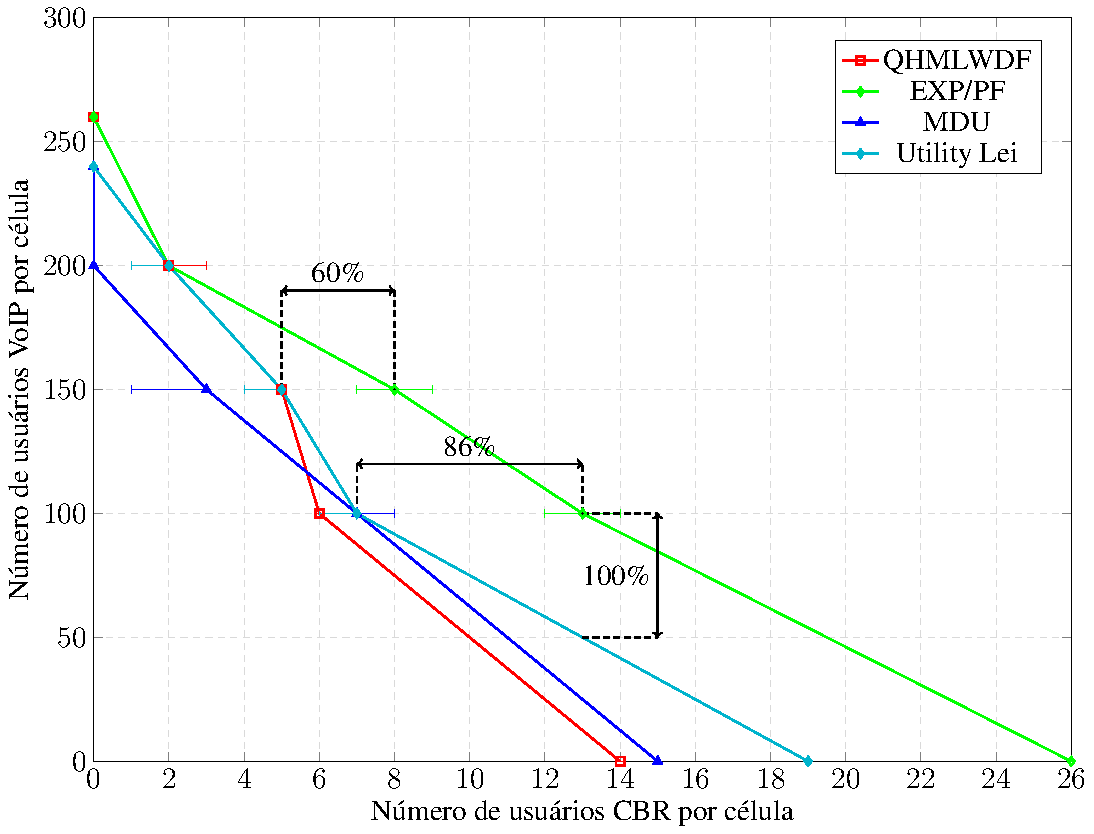
\includegraphics[width=1\linewidth]{figs/CapacityPlane.pdf}
	
	\legend{Fonte: Elaborada pelo autor.}
	\label{fig:CapPlane}
\end{figure}

Em segundo lugar ficou o \textit{Utility} Lei, que obteve o segundo melhor desempenho em todos cenários analisados. Perceba que para este algoritmo, o intervalo de confiança mostra que existe a possibilidade de este algoritmo obter desempenho igual ou pior que o desempenho do QHMLWDF nos cenários analisados, o que poderia alterar a ordem de classificação dos algoritmos segundo seus desempenhos. O principal motivo para este algoritmo não ter conseguido atingir os mesmos resultados que o EXP/PF é que alocação dos recursos para o serviço NRT é também baseada em atraso, assim como para o serviço RT, e não baseada em vazão de dados, como feito no EXP/PF.
 
Nos dois últimos lugares ficaram os algoritmos QHMLWDF e MDU. Estes algoritmos apresentaram os dois piores desempenhos para o cenário com serviço único NRT. Em relação ao cenários com múltiplos serviços, esses algoritmos apresentaram os piores desempenhos. Em relação ao QHMLWDF, isso ocorreu pelo fato de este algoritmo utilizar o tamanho da fila para fazer a alocação de recursos, o que prejudicou bastante o nível de satisfação do serviço RT, já que a taxa de geração de pacotes do serviço CBR é maior que a do serviço VoIP. Em relação ao algoritmo MDU, o principal motivo foi que a prioridade do serviço RT era absolutamente maior que a prioridade do serviço NRT, o que fez com a satisfação do serviço NRT ficasse bastante degradada, como exemplificado na figura \ref{fig:200VOIP}, em que a satisfação do serviço NRT não ficou acima de 90\% para nenhuma carga de usuários CBR. Além disso, note que para o MDU, o intervalo de confiança dos resultados mostra que o desempenho deste algoritmo pode ser ainda significativamente pior no cenário como 150 usuários VoIP, fazendo com que este algoritmo apresente desempenho global ainda pior. 

A conclusão que pode ser obtida a partir deste resultado é que a melhor abordagem que pode ser utilizada para realizar a alocação de recursos em um cenário composto por serviços NRT e RT é a abordagem do EXP/PF, que foi: alocar os recursos para o serviço RT utilizando a métrica de atraso do pacote HOL de cada usuário e alocar os recursos para serviços NRT utilizando a métrica de vazão de dados. Essa abordagem ataca diretamente a métrica de QoS que define a satisfação de cada classe de serviço.

\chapter[Conclusões e Trabalhos Futuros]{Conclusões e Trabalhos Futuros}
% ----------------------------------------------------------

Este trabalho apresentou um estudo de quatro algoritmos de alocação de recursos de rádio para múltiplos serviços em redes celulares LTE de 4G baseadas em OFDMA, em que os quatro algoritmos foram escolhidos após uma extensão revisão bibliográfica. O estudo destes algoritmos se deu por meio da implementação de tais algoritmos para análise de desempenho com base na métrica de satisfação do usuário. O ambiente de simulação modelado e utilizado neste trabalho era composto por dois tipos de serviço: serviço CBR, o qual pode ser classificado como NRT, e o serviço VoIP, que é um serviço RT. 

A avaliação do desempenho dos quatro algoritmos estudados se deu por meio de simulações em ambientes com serviço único RT, serviço único NRT e múltiplos serviços. A partir dos resultados destas simulações, foram obtidas as cargas de usuários tal que o nível de satisfação dos usuários estava acima de 90\%. Esses valores foram então utilizados para a construção do plano de capacidade, que nos permite condensar o desempenho de todos os algoritmos em todos os cenários em um único gráfico. Note que com isso, todos os objetivos inicialmente estabelecidos para este trabalho foram atingidos. 

A partir da análise do desempenho dos algoritmos em todos estes cenários, conclui-se que o algoritmo que obteve o melhor foi o EXP/PF, já que ele obteve os melhores resultados para todos os cenários com serviço único e múltiplos serviços. O motivo para isso é que este algoritmo faz a alocação dos recursos para os serviços RT e NRT com base na principal métrica de QoS que define se os usuários destes serviços estão satisfeitos. O segundo melhor desempenho foi obtido pelo algoritmo \textit{Utility} Lei, o qual obteve o segundo melhor desempenho em todos os cenários analisados. A principal desvantagem do \textit{Utility} Lei é que ele aloca os recursos para as duas classes de serviço com base na métrica de atraso do pacote HOL, em vez de focar na alocação baseada em vazão de dados para o serviço NRT. Os dois piores desempenhos foram obtidos pelos algoritmos MDU e QHMLWDF. Em relação ao MDU, o principal motivo para o baixo desempenho é a maior prioridade absoluta dada para o serviço RT, o que deteriora a satisfação do serviço NRT. O QHMLWDF atingiu tão baixo desempenho pelo fato de utilizar o tamanho da fila absoluto para alocar os recursos para os dois serviços, o que prejudicou o seu desempenho pelo fato de os serviços analisados possuírem taxas de geração de pacotes bastantes distintas.   

Conclui-se, portanto, que os algoritmos de RRA são mecanismos que já foram e continuam sendo bastante estudados por pesquisadores da área das telecomunicações, como percebido pelo que foi apresentado no segundo capítulo. Pode-se concluir também que há diversas formas para formular/conceber algoritmos de RRA, desde abordagens heurísticas/experimentais até abordagens com uma sólida formulação matemática baseada em alguma teoria, tal como a teoria da utilidade. 

Segundo \citeonline{kim2009qos}, uma característica desejada que poderia estar presente em algoritmos de RRA é a flexibilidade para que as operadoras das redes celulares ajustem o ponto de operação dos algoritmos de acordo com decisões estratégicas ou segundo as mudanças de tendências dos clientes. Um ajuste de operação que poderia ser tomado de acordo com decisões estratégicas é dar maior prioridade para o serviço que gera maior quantidade de tráfego, o que resultaria em um aumento da vazão de dados total do sistema. Em relação as mudanças na tendência dos clientes, uma decisão que poderia ser tomada é atribuir maior prioridade para um determinado serviço que está sendo utilizado pela maioria dos usuários presentes no sistema. Nenhum dos algoritmos estudados aqui e nenhum outro algoritmo que foi encontrado na literatura se preocupa com este tipo de característica, o que abre espaço para possíveis trabalhos futuros.

Por fim, devido a essa grande área de pesquisa que é o estudo de algoritmos de RRA, existe a perspectiva que em trabalhos futuros do autor um algoritmo de RRA seja desenvolvido para ser aplicado em redes celulares 4G e 5ª Geração (5G) com múltiplos serviços. Pode-se adotar uma abordagem que possua uma fundamentação matemática ou mesmo uma abordagem heurística que seja eficaz. Como nenhum dos algoritmos apresentados aqui se preocupou com o que foi exposto em \citeonline{kim2009qos}, o algoritmo de RRA a ser desenvolvido deveria atender a este critério. Uma alternativa para isso é permitir que as operadoras de redes celulares tivessem a possibilidade de escolher um serviço para ter maior prioridade sobre o outro, em que o serviço protegido poderia permanecer com o nível de satisfação do usuário sempre acima de um limiar pré-determinado. Tal característica poderia ser alcança utilizando algum mecanismo de controle de satisfação feito de forma dinâmica, ou seja, em tempo de execução. Pode-se também investigar outras classes de serviços que tornem o cenário mais desafiador para os algoritmos de RRA, além de analisar o desempenho dos algoritmos em ambientes com múltiplas células, o que torna o cenário ainda mais desafiador devido a presença da interferência gerada por uma célula em células vizinhas. Para finalizar, devido a grande quantidade de usuários que está projetada para acessar as redes celulares 5G e a grande quantidade de dados que usuários vão demandar \cite{osseiran2014scenarios}, vale ressaltar que para que o algoritmo a ser desenvolvido possa ser aplicado em redes celulares 5G, é necessário que ele seja capaz de gerenciar de forma bastante eficiente os recursos de rádio para que os requerimentos de QoS dos usuários conectados sejam atendidos.
	
% Capitulo com exemplos de comandos inseridos de arquivo externo 
%%% abtex2-modelo-include-comandos.tex, v<VERSION> laurocesar
%% Copyright 2012-<COPYRIGHT_YEAR> by abnTeX2 group at http://www.abntex.net.br/ 
%%
%% This work may be distributed and/or modified under the
%% conditions of the LaTeX Project Public License, either version 1.3
%% of this license or (at your option) any later version.
%% The latest version of this license is in
%%   http://www.latex-project.org/lppl.txt
%% and version 1.3 or later is part of all distributions of LaTeX
%% version 2005/12/01 or later.
%%
%% This work has the LPPL maintenance status `maintained'.
%% 
%% The Current Maintainer of this work is the abnTeX2 team, led
%% by Lauro César Araujo. Further information are available on 
%% http://www.abntex.net.br/
%%
%% This work consists of the files abntex2-modelo-include-comandos.tex
%% and abntex2-modelo-img-marca.pdf
%%

% ---
% Este capítulo, utilizado por diferentes exemplos do abnTeX2, ilustra o uso de
% comandos do abnTeX2 e de LaTeX.
% ---
 
\chapter{Resultados de comandos}\label{cap_exemplos}

\chapterprecis{Isto é uma sinopse de capítulo. A ABNT não traz nenhuma
normatização a respeito desse tipo de resumo, que é mais comum em romances 
e livros técnicos.}\index{sinopse de capítulo}

% ---
\section{Codificação dos arquivos: UTF8}
% ---

A codificação de todos os arquivos do \abnTeX\ é \texttt{UTF8}. É necessário que
você utilize a mesma codificação nos documentos que escrever, inclusive nos
arquivos de base bibliográficas |.bib|.

% ---
\section{Citações diretas}
\label{sec-citacao}
% ---

\index{citações!diretas}Utilize o ambiente \texttt{citacao} para incluir
citações diretas com mais de três linhas:

\begin{citacao}
As citações diretas, no texto, com mais de três linhas, devem ser
destacadas com recuo de 4 cm da margem esquerda, com letra menor que a do texto
utilizado e sem as aspas. No caso de documentos datilografados, deve-se
observar apenas o recuo \cite[5.3]{NBR10520:2002}.
\end{citacao}

Use o ambiente assim:

\begin{verbatim}
\begin{citacao}
As citações diretas, no texto, com mais de três linhas [...] deve-se observar
apenas o recuo \cite[5.3]{NBR10520:2002}.
\end{citacao}
\end{verbatim}

O ambiente \texttt{citacao} pode receber como parâmetro opcional um nome de
idioma previamente carregado nas opções da classe (\autoref{sec-hifenizacao}). Nesse
caso, o texto da citação é automaticamente escrito em itálico e a hifenização é
ajustada para o idioma selecionado na opção do ambiente. Por exemplo:

\begin{verbatim}
\begin{citacao}[english]
Text in English language in italic with correct hyphenation.
\end{citacao}
\end{verbatim}

Tem como resultado:

\begin{citacao}[english]
Text in English language in italic with correct hyphenation.
\end{citacao}

\index{citações!simples}Citações simples, com até três linhas, devem ser
incluídas com aspas. Observe que em \LaTeX as aspas iniciais são diferentes das
finais: ``Amor é fogo que arde sem se ver''.

% ---
\section{Notas de rodapé}
% ---

As notas de rodapé são detalhadas pela NBR 14724:2011 na seção 5.2.1\footnote{As
notas devem ser digitadas ou datilografadas dentro das margens, ficando
separadas do texto por um espaço simples de entre as linhas e por filete de 5
cm, a partir da margem esquerda. Devem ser alinhadas, a partir da segunda linha
da mesma nota, abaixo da primeira letra da primeira palavra, de forma a destacar
o expoente, sem espaço entre elas e com fonte menor
\citeonline[5.2.1]{NBR14724:2011}.}\footnote{Caso uma série de notas sejam
criadas sequencialmente, o \abnTeX\ instrui o \LaTeX\ para que uma vírgula seja
colocada após cada número do expoente que indica a nota de rodapé no corpo do
texto.}\footnote{Verifique se os números do expoente possuem uma vírgula para
dividi-los no corpo do texto.}. 


% ---
\section{Tabelas}
% ---

\index{tabelas}A \autoref{tab-nivinv} é um exemplo de tabela construída em
\LaTeX.

\begin{table}[htb]
\ABNTEXfontereduzida
\caption[Níveis de investigação]{Níveis de investigação.}
\label{tab-nivinv}
\begin{tabular}{p{2.6cm}|p{6.0cm}|p{2.25cm}|p{3.40cm}}
  %\hline
   \textbf{Nível de Investigação} & \textbf{Insumos}  & \textbf{Sistemas de Investigação}  & \textbf{Produtos}  \\
    \hline
    Meta-nível & Filosofia\index{filosofia} da Ciência  & Epistemologia &
    Paradigma  \\
    \hline
    Nível do objeto & Paradigmas do metanível e evidências do nível inferior &
    Ciência  & Teorias e modelos \\
    \hline
    Nível inferior & Modelos e métodos do nível do objeto e problemas do nível inferior & Prática & Solução de problemas  \\
   % \hline
\end{tabular}
\legend{Fonte: \citeonline{van86}}
\end{table}

Já a \autoref{tabela-ibge} apresenta uma tabela criada conforme o padrão do
\citeonline{ibge1993} requerido pelas normas da ABNT para documentos técnicos e
acadêmicos.

\begin{table}[htb]
\IBGEtab{%
  \caption{Um Exemplo de tabela alinhada que pode ser longa
  ou curta, conforme padrão IBGE.}%
  \label{tabela-ibge}
}{%
  \begin{tabular}{ccc}
  \toprule
   Nome & Nascimento & Documento \\
  \midrule \midrule
   Maria da Silva & 11/11/1111 & 111.111.111-11 \\
  \midrule 
   João Souza & 11/11/2111 & 211.111.111-11 \\
  \midrule 
   Laura Vicuña & 05/04/1891 & 3111.111.111-11 \\
  \bottomrule
\end{tabular}%
}{%
  \fonte{Produzido pelos autores.}%
  \nota{Esta é uma nota, que diz que os dados são baseados na
  regressão linear.}%
  \nota[Anotações]{Uma anotação adicional, que pode ser seguida de várias
  outras.}%
  }
\end{table}


% ---
\section{Figuras}
% ---

\index{figuras}Figuras podem ser criadas diretamente em \LaTeX,
como o exemplo da \autoref{fig_circulo}.

\begin{figure}[htb]
	\caption{\label{fig_circulo}A delimitação do espaço}
	\begin{center}
	    \setlength{\unitlength}{5cm}
		\begin{picture}(1,1)
		\put(0,0){\line(0,1){1}}
		\put(0,0){\line(1,0){1}}
		\put(0,0){\line(1,1){1}}
		\put(0,0){\line(1,2){.5}}
		\put(0,0){\line(1,3){.3333}}
		\put(0,0){\line(1,4){.25}}
		\put(0,0){\line(1,5){.2}}
		\put(0,0){\line(1,6){.1667}}
		\put(0,0){\line(2,1){1}}
		\put(0,0){\line(2,3){.6667}}
		\put(0,0){\line(2,5){.4}}
		\put(0,0){\line(3,1){1}}
		\put(0,0){\line(3,2){1}}
		\put(0,0){\line(3,4){.75}}
		\put(0,0){\line(3,5){.6}}
		\put(0,0){\line(4,1){1}}
		\put(0,0){\line(4,3){1}}
		\put(0,0){\line(4,5){.8}}
		\put(0,0){\line(5,1){1}}
		\put(0,0){\line(5,2){1}}
		\put(0,0){\line(5,3){1}}
		\put(0,0){\line(5,4){1}}
		\put(0,0){\line(5,6){.8333}}
		\put(0,0){\line(6,1){1}}
		\put(0,0){\line(6,5){1}}
		\end{picture}
	\end{center}
	\legend{Fonte: os autores}
\end{figure}

Ou então figuras podem ser incorporadas de arquivos externos, como é o caso da
\autoref{fig_grafico}. Se a figura que ser incluída se tratar de um diagrama, um
gráfico ou uma ilustração que você mesmo produza, priorize o uso de imagens
vetoriais no formato PDF. Com isso, o tamanho do arquivo final do trabalho será
menor, e as imagens terão uma apresentação melhor, principalmente quando
impressas, uma vez que imagens vetorias são perfeitamente escaláveis para
qualquer dimensão. Nesse caso, se for utilizar o Microsoft Excel para produzir
gráficos, ou o Microsoft Word para produzir ilustrações, exporte-os como PDF e
os incorpore ao documento conforme o exemplo abaixo. No entanto, para manter a
coerência no uso de software livre (já que você está usando \LaTeX e \abnTeX),
teste a ferramenta \textsf{InkScape}\index{InkScape}
(\url{http://inkscape.org/}). Ela é uma excelente opção de código-livre para
produzir ilustrações vetoriais, similar ao CorelDraw\index{CorelDraw} ou ao Adobe
Illustrator\index{Adobe Illustrator}. De todo modo, caso não seja possível
utilizar arquivos de imagens como PDF, utilize qualquer outro formato, como
JPEG, GIF, BMP, etc. Nesse caso, você pode tentar aprimorar as imagens
incorporadas com o software livre \textsf{Gimp}\index{Gimp}
(\url{http://www.gimp.org/}). Ele é uma alternativa livre ao Adobe
Photoshop\index{Adobe Photoshop}.

\begin{figure}[htb]
	\caption{\label{fig_grafico}Gráfico produzido em Excel e salvo como PDF}
	\begin{center}
	    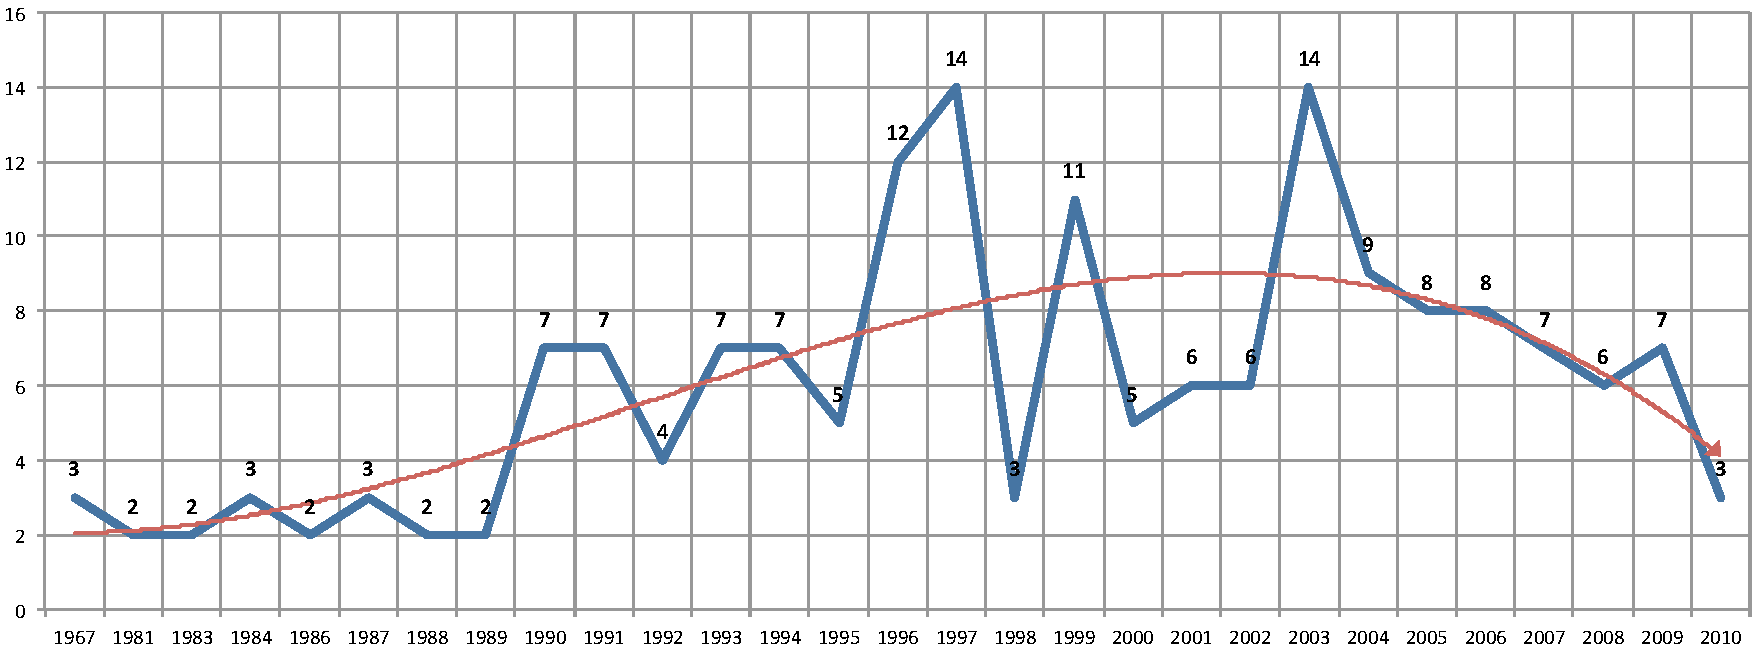
\includegraphics[scale=0.5]{abntex2-modelo-img-grafico.pdf}
	\end{center}
	\legend{Fonte: \citeonline[p. 24]{araujo2012}}
\end{figure}

% ---
\subsection{Figuras em \emph{minipages}}
% ---

\emph{Minipages} são usadas para inserir textos ou outros elementos em quadros
com tamanhos e posições controladas. Veja o exemplo da
\autoref{fig_minipage_imagem1} e da \autoref{fig_minipage_grafico2}.

\begin{figure}[htb]
 \label{teste}
 \centering
  \begin{minipage}{0.4\textwidth}
    \centering
    \caption{Imagem 1 da minipage} \label{fig_minipage_imagem1}
    
\includegraphics[scale=0.9]{abntex2-modelo-img-marca.pdf}
    \legend{Fonte: Produzido pelos autores}
  \end{minipage}
  \hfill
  \begin{minipage}{0.4\textwidth}
    \centering
    \caption{Grafico 2 da minipage} \label{fig_minipage_grafico2}
    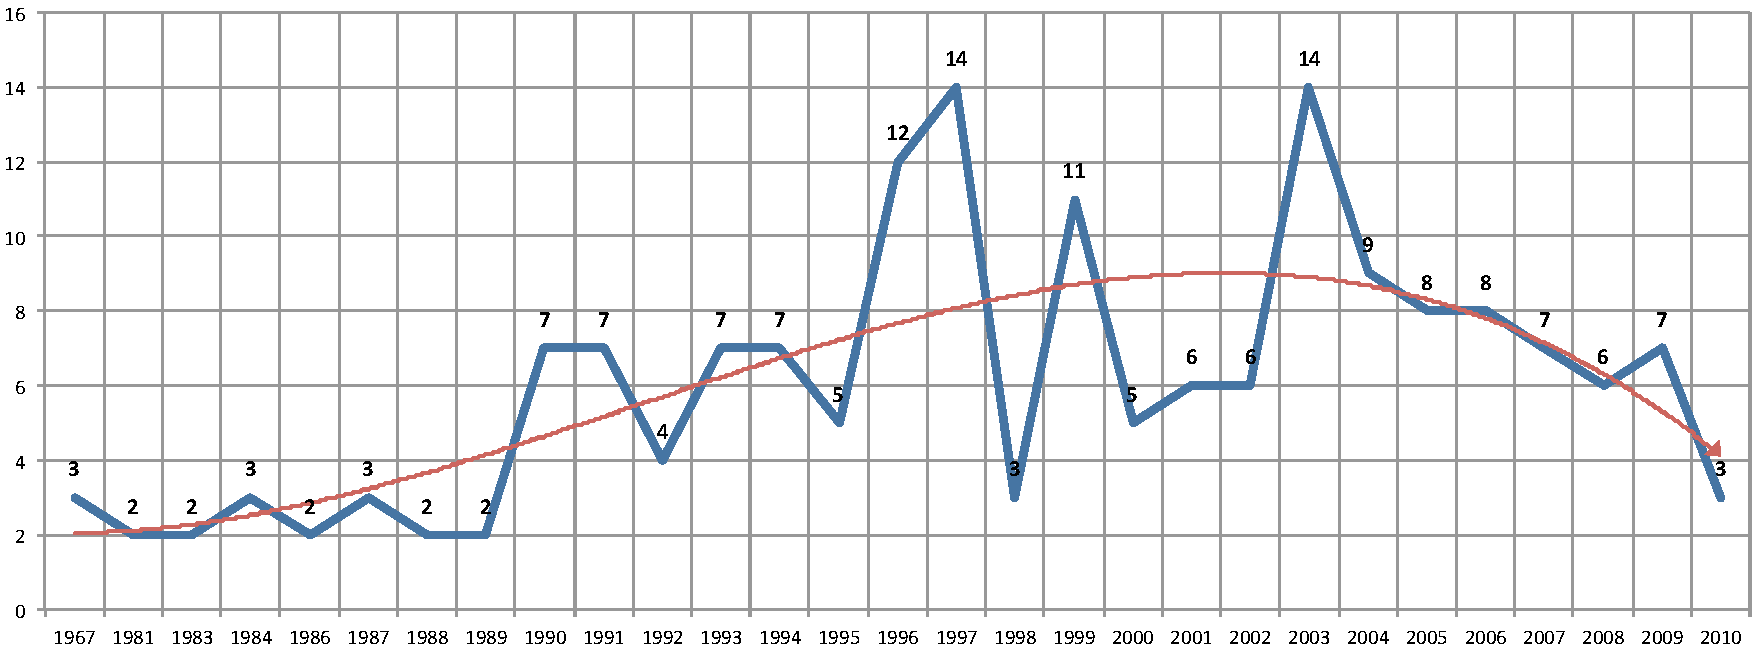
\includegraphics[scale=0.2]{abntex2-modelo-img-grafico.pdf}
    \legend{Fonte: \citeonline[p. 24]{araujo2012}}
  \end{minipage}
\end{figure}

Observe que, segundo a \citeonline[seções 4.2.1.10 e 5.8]{NBR14724:2011}, as
ilustrações devem sempre ter numeração contínua e única em todo o documento:

\begin{citacao}
Qualquer que seja o tipo de ilustração, sua identificação aparece na parte
superior, precedida da palavra designativa (desenho, esquema, fluxograma,
fotografia, gráfico, mapa, organograma, planta, quadro, retrato, figura,
imagem, entre outros), seguida de seu número de ordem de ocorrência no texto,
em algarismos arábicos, travessão e do respectivo título. Após a ilustração, na
parte inferior, indicar a fonte consultada (elemento obrigatório, mesmo que
seja produção do próprio autor), legenda, notas e outras informações
necessárias à sua compreensão (se houver). A ilustração deve ser citada no
texto e inserida o mais próximo possível do trecho a que se
refere. \cite[seções 5.8]{NBR14724:2011}
\end{citacao}

% ---
\section{Expressões matemáticas}
% ---

\index{expressões matemáticas}Use o ambiente \texttt{equation} para escrever
expressões matemáticas numeradas:

\begin{equation}
  \forall x \in X, \quad \exists \: y \leq \epsilon
\end{equation}

Escreva expressões matemáticas entre \$ e \$, como em $ \lim_{x \to \infty}
\exp(-x) = 0 $, para que fiquem na mesma linha.

Também é possível usar colchetes para indicar o início de uma expressão
matemática que não é numerada.

\[
\left|\sum_{i=1}^n a_ib_i\right|
\le
\left(\sum_{i=1}^n a_i^2\right)^{1/2}
\left(\sum_{i=1}^n b_i^2\right)^{1/2}
\]

Consulte mais informações sobre expressões matemáticas em
\url{https://github.com/abntex/abntex2/wiki/Referencias}.

% ---
\section{Enumerações: alíneas e subalíneas}
% ---

\index{alíneas}\index{subalíneas}\index{incisos}Quando for necessário enumerar
os diversos assuntos de uma seção que não possua título, esta deve ser
subdividida em alíneas \cite[4.2]{NBR6024:2012}:

\begin{alineas}

  \item os diversos assuntos que não possuam título próprio, dentro de uma mesma
  seção, devem ser subdivididos em alíneas; 
  
  \item o texto que antecede as alíneas termina em dois pontos;
  \item as alíneas devem ser indicadas alfabeticamente, em letra minúscula,
  seguida de parêntese. Utilizam-se letras dobradas, quando esgotadas as
  letras do alfabeto;

  \item as letras indicativas das alíneas devem apresentar recuo em relação à
  margem esquerda;

  \item o texto da alínea deve começar por letra minúscula e terminar em
  ponto-e-vírgula, exceto a última alínea que termina em ponto final;

  \item o texto da alínea deve terminar em dois pontos, se houver subalínea;

  \item a segunda e as seguintes linhas do texto da alínea começa sob a
  primeira letra do texto da própria alínea;
  
  \item subalíneas \cite[4.3]{NBR6024:2012} devem ser conforme as alíneas a
  seguir:

  \begin{alineas}
     \item as subalíneas devem começar por travessão seguido de espaço;

     \item as subalíneas devem apresentar recuo em relação à alínea;

     \item o texto da subalínea deve começar por letra minúscula e terminar em
     ponto-e-vírgula. A última subalínea deve terminar em ponto final, se não
     houver alínea subsequente;

     \item a segunda e as seguintes linhas do texto da subalínea começam sob a
     primeira letra do texto da própria subalínea.
  \end{alineas}
  
  \item no \abnTeX\ estão disponíveis os ambientes \texttt{incisos} e
  \texttt{subalineas}, que em suma são o mesmo que se criar outro nível de
  \texttt{alineas}, como nos exemplos à seguir:
  
  \begin{incisos}
    \item \textit{Um novo inciso em itálico};
  \end{incisos}
  
  \item Alínea em \textbf{negrito}:
  
  \begin{subalineas}
    \item \textit{Uma subalínea em itálico};
    \item \underline{\textit{Uma subalínea em itálico e sublinhado}}; 
  \end{subalineas}
  
  \item Última alínea com \emph{ênfase}.
  
\end{alineas}

% ---
\section{Espaçamento entre parágrafos e linhas}
% ---

\index{espaçamento!dos parágrafos}O tamanho do parágrafo, espaço entre a margem
e o início da frase do parágrafo, é definido por:

\begin{verbatim}
   \setlength{\parindent}{1.3cm}
\end{verbatim}

\index{espaçamento!do primeiro parágrafo}Por padrão, não há espaçamento no
primeiro parágrafo de cada início de divisão do documento
(\autoref{sec-divisoes}). Porém, você pode definir que o primeiro parágrafo
também seja indentado, como é o caso deste documento. Para isso, apenas inclua o
pacote \textsf{indentfirst} no preâmbulo do documento:

\begin{verbatim}
   \usepackage{indentfirst}      % Indenta o primeiro parágrafo de cada seção.
\end{verbatim}

\index{espaçamento!entre os parágrafos}O espaçamento entre um parágrafo e outro
pode ser controlado por meio do comando:

\begin{verbatim}
  \setlength{\parskip}{0.2cm}  % tente também \onelineskip
\end{verbatim}

\index{espaçamento!entre as linhas}O controle do espaçamento entre linhas é
definido por:

\begin{verbatim}
  \OnehalfSpacing       % espaçamento um e meio (padrão); 
  \DoubleSpacing        % espaçamento duplo
  \SingleSpacing        % espaçamento simples	
\end{verbatim}

Para isso, também estão disponíveis os ambientes:

\begin{verbatim}
  \begin{SingleSpace} ...\end{SingleSpace}
  \begin{Spacing}{hfactori} ... \end{Spacing}
  \begin{OnehalfSpace} ... \end{OnehalfSpace}
  \begin{OnehalfSpace*} ... \end{OnehalfSpace*}
  \begin{DoubleSpace} ... \end{DoubleSpace}
  \begin{DoubleSpace*} ... \end{DoubleSpace*} 
\end{verbatim}

Para mais informações, consulte \citeonline[p. 47-52 e 135]{memoir}.

% ---
\section{Inclusão de outros arquivos}\label{sec-include}
% ---

É uma boa prática dividir o seu documento em diversos arquivos, e não
apenas escrever tudo em um único. Esse recurso foi utilizado neste
documento. Para incluir diferentes arquivos em um arquivo principal,
de modo que cada arquivo incluído fique em uma página diferente, utilize o
comando:

\begin{verbatim}
   \include{documento-a-ser-incluido}      % sem a extensão .tex
\end{verbatim}

Para incluir documentos sem quebra de páginas, utilize:

\begin{verbatim}
   \input{documento-a-ser-incluido}      % sem a extensão .tex
\end{verbatim}

% ---
\section{Compilar o documento \LaTeX}
% ---

Geralmente os editores \LaTeX, como o
TeXlipse\footnote{\url{http://texlipse.sourceforge.net/}}, o
Texmaker\footnote{\url{http://www.xm1math.net/texmaker/}}, entre outros,
compilam os documentos automaticamente, de modo que você não precisa se
preocupar com isso.

No entanto, você pode compilar os documentos \LaTeX usando os seguintes
comandos, que devem ser digitados no \emph{Prompt de Comandos} do Windows ou no
\emph{Terminal} do Mac ou do Linux:

\begin{verbatim}
   pdflatex ARQUIVO_PRINCIPAL.tex
   bibtex ARQUIVO_PRINCIPAL.aux
   makeindex ARQUIVO_PRINCIPAL.idx 
   makeindex ARQUIVO_PRINCIPAL.nlo -s nomencl.ist -o ARQUIVO_PRINCIPAL.nls
   pdflatex ARQUIVO_PRINCIPAL.tex
   pdflatex ARQUIVO_PRINCIPAL.tex
\end{verbatim}

% ---
\section{Remissões internas}
% ---

Ao nomear a \autoref{tab-nivinv} e a \autoref{fig_circulo}, apresentamos um
exemplo de remissão interna, que também pode ser feita quando indicamos o
\autoref{cap_exemplos}, que tem o nome \emph{\nameref{cap_exemplos}}. O número
do capítulo indicado é \ref{cap_exemplos}, que se inicia à
\autopageref{cap_exemplos}\footnote{O número da página de uma remissão pode ser
obtida também assim:
\pageref{cap_exemplos}.}.
Veja a \autoref{sec-divisoes} para outros exemplos de remissões internas entre
seções, subseções e subsubseções.

O código usado para produzir o texto desta seção é:

\begin{verbatim}
Ao nomear a \autoref{tab-nivinv} e a \autoref{fig_circulo}, apresentamos um
exemplo de remissão interna, que também pode ser feita quando indicamos o
\autoref{cap_exemplos}, que tem o nome \emph{\nameref{cap_exemplos}}. O número
do capítulo indicado é \ref{cap_exemplos}, que se inicia à
\autopageref{cap_exemplos}\footnote{O número da página de uma remissão pode ser
obtida também assim:
\pageref{cap_exemplos}.}.
Veja a \autoref{sec-divisoes} para outros exemplos de remissões internas entre
seções, subseções e subsubseções.
\end{verbatim}

% ---
\section{Divisões do documento: seção}\label{sec-divisoes}
% ---

Esta seção testa o uso de divisões de documentos. Esta é a
\autoref{sec-divisoes}. Veja a \autoref{sec-divisoes-subsection}.

\subsection{Divisões do documento: subseção}\label{sec-divisoes-subsection}

Isto é uma subseção. Veja a \autoref{sec-divisoes-subsubsection}, que é uma
\texttt{subsubsection} do \LaTeX, mas é impressa chamada de ``subseção'' porque
no Português não temos a palavra ``subsubseção''.

\subsubsection{Divisões do documento: subsubseção}
\label{sec-divisoes-subsubsection}

Isto é uma subsubseção.

\subsubsection{Divisões do documento: subsubseção}

Isto é outra subsubseção.

\subsection{Divisões do documento: subseção}\label{sec-exemplo-subsec}

Isto é uma subseção.

\subsubsection{Divisões do documento: subsubseção}

Isto é mais uma subsubseção da \autoref{sec-exemplo-subsec}.


\subsubsubsection{Esta é uma subseção de quinto
nível}\label{sec-exemplo-subsubsubsection}

Esta é uma seção de quinto nível. Ela é produzida com o seguinte comando:

\begin{verbatim}
\subsubsubsection{Esta é uma subseção de quinto
nível}\label{sec-exemplo-subsubsubsection}
\end{verbatim}

\subsubsubsection{Esta é outra subseção de quinto nível}\label{sec-exemplo-subsubsubsection-outro}

Esta é outra seção de quinto nível.


\paragraph{Este é um parágrafo numerado}\label{sec-exemplo-paragrafo}

Este é um exemplo de parágrafo nomeado. Ele é produzida com o comando de
parágrafo:

\begin{verbatim}
\paragraph{Este é um parágrafo nomeado}\label{sec-exemplo-paragrafo}
\end{verbatim}

A numeração entre parágrafos numeradaos e subsubsubseções são contínuas.

\paragraph{Esta é outro parágrafo numerado}\label{sec-exemplo-paragrafo-outro}

Esta é outro parágrafo nomeado.

% ---
\section{Este é um exemplo de nome de seção longo. Ele deve estar
alinhado à esquerda e a segunda e demais linhas devem iniciar logo abaixo da
primeira palavra da primeira linha}
% ---

Isso atende à norma \citeonline[seções de 5.2.2 a 5.2.4]{NBR14724:2011} 
 e \citeonline[seções de 3.1 a 3.8]{NBR6024:2012}.

% ---
\section{Diferentes idiomas e hifenizações}
\label{sec-hifenizacao}
% ---

Para usar hifenizações de diferentes idiomas, inclua nas opções do documento o
nome dos idiomas que o seu texto contém. Por exemplo (para melhor
visualização, as opções foram quebras em diferentes linhas):

\begin{verbatim}
\documentclass[
	12pt,
	openright,
	twoside,
	a4paper,
	english,
	brazil
	]{abntex2}
\end{verbatim}

O idioma português-brasileiro (\texttt{brazil}) é incluído automaticamente pela
classe \textsf{abntex2}. Porém, mesmo assim a opção \texttt{brazil} deve ser
informada como a última opção da classe para que todos os pacotes reconheçam o
idioma. Vale ressaltar que a última opção de idioma é a utilizada por padrão no
documento. Desse modo, caso deseje escrever um texto em inglês que tenha
citações em português e em francês, você deveria usar o preâmbulo como abaixo:

\begin{verbatim}
\documentclass[
	12pt,
	openright,
	twoside,
	a4paper,
	brazil,
	english
	]{abntex2}
\end{verbatim}

A lista completa de idiomas suportados, bem como outras opções de hifenização,
estão disponíveis em \citeonline[p.~5-6]{babel}.

Exemplo de hifenização em inglês\footnote{Extraído de:
\url{http://en.wikibooks.org/wiki/LaTeX/Internationalization}}:

\begin{otherlanguage*}{english}
\textit{Text in English language. This environment switches all language-related
definitions, like the language specific names for figures, tables etc. to the other
language. The starred version of this environment typesets the main text
according to the rules of the other language, but keeps the language specific
string for ancillary things like figures, in the main language of the document.
The environment hyphenrules switches only the hyphenation patterns used; it can
also be used to disallow hyphenation by using the language name
`nohyphenation'.}
\end{otherlanguage*}

Exemplo de hifenização em francês\footnote{Extraído de:
\url{http://bigbrowser.blog.lemonde.fr/2013/02/17/tu-ne-tweeteras-point-le-vatican-interdit-aux-cardinaux-de-tweeter-pendant-le-conclave/}}:

Pequeno texto em espanhol\footnote{Extraído de:
\url{http://internacional.elpais.com/internacional/2013/02/17/actualidad/1361102009_913423.html}}:

O idioma geral do texto por ser alterado como no exemplo seguinte:

\begin{verbatim}
  \selectlanguage{english}
\end{verbatim}

Isso altera automaticamente a hifenização e todos os nomes constantes de
referências do documento para o idioma inglês. Consulte o manual da classe
\cite{abntex2classe} para obter orientações adicionais sobre internacionalização de
documentos produzidos com \abnTeX.

A \autoref{sec-citacao} descreve o ambiente \texttt{citacao} que pode receber
como parâmetro um idioma a ser usado na citação.

% ---
\section{Consulte o manual da classe \textsf{abntex2}}
% ---

Consulte o manual da classe \textsf{abntex2} \cite{abntex2classe} para uma
referência completa das macros e ambientes disponíveis. 

Além disso, o manual possui informações adicionais sobre as normas ABNT
observadas pelo \abnTeX\ e considerações sobre eventuais requisitos específicos
não atendidos, como o caso da \citeonline[seção 5.2.2]{NBR14724:2011}, que
especifica o espaçamento entre os capítulos e o início do texto, regra
propositalmente não atendida pelo presente modelo.

% ---
\section{Referências bibliográficas}
% ---

A formatação das referências bibliográficas conforme as regras da ABNT são um
dos principais objetivos do \abnTeX. Consulte os manuais
\citeonline{abntex2cite} e \citeonline{abntex2cite-alf} para obter informações
sobre como utilizar as referências bibliográficas.

%-
\subsection{Acentuação de referências bibliográficas}
%-

Normalmente não há problemas em usar caracteres acentuados em arquivos
bibliográficos (\texttt{*.bib}). Porém, como as regras da ABNT fazem uso quase
abusivo da conversão para letras maiúsculas, é preciso observar o modo como se
escreve os nomes dos autores. Na ~\autoref{tabela-acentos} você encontra alguns
exemplos das conversões mais importantes. Preste atenção especial para `ç' e `í'
que devem estar envoltos em chaves. A regra geral é sempre usar a acentuação
neste modo quando houver conversão para letras maiúsculas.

\begin{table}[htbp]
\caption{Tabela de conversão de acentuação.}
\label{tabela-acentos}

\begin{center}
\begin{tabular}{ll}\hline\hline
acento & \textsf{bibtex}\\
à á ã & \verb+\`a+ \verb+\'a+ \verb+\~a+\\
í & \verb+{\'\i}+\\
ç & \verb+{\c c}+\\
\hline\hline
\end{tabular}
\end{center}
\end{table}


% ---
\section{Precisa de ajuda?}
% ---

Consulte a FAQ com perguntas frequentes e comuns no portal do \abnTeX:
\url{https://github.com/abntex/abntex2/wiki/FAQ}.

Inscreva-se no grupo de usuários \LaTeX:
\url{http://groups.google.com/group/latex-br}, tire suas dúvidas e ajude
outros usuários.

Participe também do grupo de desenvolvedores do \abnTeX:
\url{http://groups.google.com/group/abntex2} e faça sua contribuição à
ferramenta.

% ---
\section{Você pode ajudar?}
% ---

Sua contribuição é muito importante! Você pode ajudar na divulgação, no
desenvolvimento e de várias outras formas. Veja como contribuir com o \abnTeX\
em \url{https://github.com/abntex/abntex2/wiki/Como-Contribuir}.

% ---
\section{Quer customizar os modelos do \abnTeX\ para sua instituição ou
universidade?}
% ---

Veja como customizar o \abnTeX\ em:
\url{https://github.com/abntex/abntex2/wiki/ComoCustomizar}.

% ----------------------------------------------------------
% ELEMENTOS PÓS-TEXTUAIS
% ----------------------------------------------------------
\postextual

% Referências bibliográficas
\bibliography{bibtex/referencias}

% Glossário (Consulte o manual da classe abntex2 para orientações sobre o glossário)
%\glossary

% Apêndices
%% Apêndices
% ---
% Inicia os apêndices
% ---
\begin{apendicesenv}
	
% ----------------------------------------------------------
\chapter{Optimization Formulation for Throughput-Based Services}
\label{Ap:ThrBasedOpt}

As explained in section \ref{subsec:cap03ThrBased}, the considered optimization problem for throughput-based services is the maximization of the total utility with respect to the users' throughput. Thus, the objective function is 
%
\begin{equation}
\label{JSM:Eq:Util_Opt_Joint_NRT_App}
\underset{\rho_{j,k},\;p_{k}}{\text{max}} \; \sum_{j \in \mathcal{J}} V\left[U_{\mathrm{thr}}\left(T_{j}\left[n\right]\right)\right],
\end{equation} 
%
where $V\left(\cdot\right)$ is the service utility function and $U_{\mathrm{thr}}\left(\cdot\right)$ is the user utility function that is associated to the \ac{UE} $j$ that uses a throughput-based service.

The throughput of user $j$ is calculated using an exponential smoothing filtering, as indicated below: 
%
\begin{equation}
\label{JSM:Eq:Util_Thru_Calc}
T_{j}\left[n\right] = \left(1 - f_{\mathrm{thru}}\right) \cdot T_{j}\left[n-1\right] + f_{\mathrm{thru}} \cdot R_j\left[n\right],
\end{equation} 
%
where $R_j\left[n\right]$ is the instantaneous data rate of user $j$ and $f_{\mathrm{thru}}$ is a filtering constant.

Evaluating the objective function in equation \eqref{JSM:Eq:Util_Opt_Joint_NRT_App} and the throughput expression in equation \eqref{JSM:Eq:Util_Thru_Calc}, the derivative of $V\left[U_{\mathrm{thr}}\left(T_{j}\right)\right]$ with respect to the transmission rate $R_j$ is given by:
%
%\begin{align}
%\label{JSM:Eq:Utility_Derivative_NRT}
%\frac{\partial V\left[U_{\mathrm{thr}}\left(T_j\right)\right]}{\partial R_j} & = \frac{\partial V}{\partial U_{\mathrm{thr}}} \cdot \frac{\partial U_{\mathrm{thr}}}{\partial T_j} \cdot \frac{\partial T_j}{\partial R_j} \notag\\
%& = \left.\dfrac{\partial V}{\partial U_{\mathrm{thr}}}\right\vert_{U_{\mathrm{thr}} = U_{\mathrm{thr}}\left(T_{j}\right)} \notag\\
%& \cdot \left.\dfrac{\partial U_{\mathrm{thr}}}{\partial T_j}\right\vert_{T_{j} = \left(1 - f_{\mathrm{thru}}\right) \cdot T_{j}\left[n-1\right] + f_{\mathrm{thru}} \cdot R_j\left[n\right]}
%\notag\\ & \cdot 	f_{\mathrm{thru}}.
%\end{align}
\begin{align}
\label{JSM:Eq:Utility_Derivative_NRT}
\frac{\partial V\left[U_{\mathrm{thr}}\left(T_j\right)\right]}{\partial R_j} & = \frac{\partial V}{\partial U_{\mathrm{thr}}} \cdot \frac{\partial U_{\mathrm{thr}}}{\partial T_j} \cdot \frac{\partial T_j}{\partial R_j} \notag\\ & = \left.\dfrac{\partial V}{\partial U_{\mathrm{thr}}}\right\vert_{U_{\mathrm{thr}} = U_{\mathrm{thr}}\left(T_{j}\right)} \cdot \left.\dfrac{\partial U_{\mathrm{thr}}}{\partial T_j}\right\vert_{T_{j} = \left(1 - f_{\mathrm{thru}}\right) \cdot T_{j}\left[n-1\right] + f_{\mathrm{thru}} \cdot R_j\left[n\right]}
\cdot f_{\mathrm{thru}}.
\end{align}

In the case that $f_{\mathrm{thru}}$ is sufficiently small, the expression above can be simplified as follows \cite{Art:Song2005_p2}:

\begin{equation}
\label{JSM:Eq:Utility_Derivative_NRT2}
\frac{\partial V\left[U_{\mathrm{thr}}\left(T_j\right)\right]}{\partial R_{j}} \approx
f_{\mathrm{thru}}
\cdot
\left.\dfrac{\partial V}{\partial U_{\mathrm{thr}}}\right\vert_{U_{\mathrm{thr}} = U_{\mathrm{thr}}\left(T_{j}\right)}
\cdot
\left.\dfrac{\partial U_{\mathrm{nrt}}}{\partial T_j}\right\vert_{T_j = T_{j}\left[n-1\right]},
\end{equation}
%
where the previous resource allocation totally determines the current values of the marginal utilities. Using the one-order Taylor formula \cite{Art:Song2005_p2, Phd:Emanuel2011} and considering equation \eqref{JSM:Eq:Utility_Derivative_NRT2}, we have
%
%\begin{align}
%\label{JSM:Eq:Taylor_NRT}
%\sum_{j \in \mathcal{J}} V\left[U_{\mathrm{thr}}\left(T_{j}\left[n\right]\right)\right] \approx &
%\sum_{j \in \mathcal{J}} V\left[U_{\mathrm{thr}}\left(T_{j}\left[n-1\right]\right)\right] \notag\\
%& + \sum_{j \in \mathcal{J}} \left.\dfrac{\partial V}{\partial U_{\mathrm{thr}}}\right\vert_{U_{\mathrm{thr}} = U_{\mathrm{thr}}\left(T_{j}\right)} \notag\\ & \cdot \left.\dfrac{\partial U_{\mathrm{thr}}}{\partial T_j}\right\vert_{T_j = T_{j}\left[n-1\right]} \notag\\ & \cdot \left(f_{\mathrm{thru}} \cdot R_j\left[n\right] - f_{\mathrm{thru}} \cdot T_j\left[n-1\right]\right).
%\end{align}
\begin{align}
\label{JSM:Eq:Taylor_NRT}
\sum_{j \in \mathcal{J}} V\left[U_{\mathrm{thr}}\left(T_{j}\left[n\right]\right)\right] \approx &
\sum_{j \in \mathcal{J}} V\left[U_{\mathrm{thr}}\left(T_{j}\left[n-1\right]\right)\right] \notag\\
& + \sum_{j \in \mathcal{J}} \left.\dfrac{\partial V}{\partial U_{\mathrm{thr}}}\right\vert_{U_{\mathrm{thr}} = U_{\mathrm{thr}}\left(T_{j}\right)} \notag \\ & \cdot \left.\dfrac{\partial U_{\mathrm{thr}}}{\partial T_j}\right\vert_{T_j = T_{j}\left[n-1\right]} \notag \\ & \cdot \left(f_{\mathrm{thru}} \cdot R_j\left[n\right] - f_{\mathrm{thru}} \cdot T_j\left[n-1\right]\right).
\end{align}

Let us consider the maximization of equation \eqref{JSM:Eq:Taylor_NRT}. Notice that the maximization of the left side of equation \eqref{JSM:Eq:Taylor_NRT} is our original optimization problem given by equation \eqref{JSM:Eq:Util_Opt_Joint_NRT_App}. The maximization of the right side of equation \eqref{JSM:Eq:Taylor_NRT} is the new simplified optimization problem. Since $f_{\mathrm{thru}}$ is a constant and $T_j\left[n-1\right]$ is known and fixed before the resource allocation at the current \ac{TTI} $n$, the new simplified optimization problem becomes linear in terms of the instantaneous user's data rate, and is given by
%
\begin{equation}
\label{JSM:Eq:Simple_Obj_Function_Thr_App}
\underset{\rho_{j,k},\;p_{k}}{\text{max}} \; \sum_{j \in \mathcal{J}} V^{'}\left(U_{\mathrm{thr}}\left(T_{j}\left[n-1\right]\right)\right) \cdot U_{\mathrm{thr}}^{'}\left(T_{j}\left[n-1\right] \right) \cdot R_{j}\left[n\right].
\end{equation}

Notice that we started with an optimization formulation based on throughput given by equation \eqref{JSM:Eq:Util_Opt_Joint_NRT_App}, made some logical assumptions and mathematical simplifications, and ended up with a linear optimization formulation based on instantaneous rates given by equation \eqref{JSM:Eq:Simple_Obj_Function_Thr_App}. According to these arguments, we claim that the instantaneous optimization maximizing equation \eqref{JSM:Eq:Simple_Obj_Function_Thr_App} leads to a long-term optimization that maximizes equation \eqref{JSM:Eq:Util_Opt_Joint_NRT_App}.

\chapter{Optimization Formulation for Delay-Based Services}
\label{Ap:DelayBasedOpt}

According to section \ref{subsec:cap03DelayBased}, the considered optimization problem for delay-based services is the maximization of the total utility with respect to the users' \ac{HOL} packet delays. The objective function is given by
%
\begin{equation}
\label{JSM:Eq:Util_Opt_Joint_QUEUE_App}
\underset{\rho_{j,k},\;p_{k}}{\text{max}} \; \sum_{j \in \mathcal{J}} V\left[U_{\mathrm{delay}}\left(d_{j}^\mathrm{hol}\left[n\right]\right)\right],
\end{equation}
%
where $V\left(\cdot\right)$ is the service utility function and $U_{\mathrm{delay}}\left(\cdot\right)$ is the user utility function that is associated to the user $j$ that makes use of a delay-based service.

In this work, we consider a recursive model for calculating an approximate value of the \ac{HOL} delay \cite{Rodrigues2014_Wiley}. The recursive equation is
%
\begin{equation}
\label{JSM:Eq:HOL_Delay}
d_{j}^\mathrm{hol}\left[n+1\right] = d_{j}^\mathrm{hol}\left[n\right] + t_{\mathrm{tti}} - \frac{1}{L} \cdot \left( \frac{R_j\left[n\right] \cdot t_{\mathrm{tti}}}{S_\mathrm{p}}\right),
\end{equation}
%
where $t_{\mathrm{tti}}$ is the duration of the \ac{TTI} in seconds, $L$ is the packet arrival rate, $S_\mathrm{p}$ is the packet size, and $R_{j}\left[n\right]$ is the instantaneous achievable transmission rate on \ac{TTI} $n$. 

Assessing the objective function in equation \eqref{JSM:Eq:Util_Opt_Joint_QUEUE_App} and the \ac{HOL} delay expression in equation \eqref{JSM:Eq:HOL_Delay}, we can see that the derivative of $V\left[U_{\mathrm{delay}}\left(d_{j}^\mathrm{hol}\right)\right]$ with respect to the transmission rate $R_j$ can be expressed as
%
%\begin{align}
%\label{JSM:Eq:Utility_Derivative_QUEUE}
%\frac{\partial V\left[U_{\mathrm{delay}}\left(d_{j}^\mathrm{hol}\right)\right]}{\partial R_j} & =
%\frac{\partial V}{\partial U_{\mathrm{delay}}}
%\cdot
%\frac{\partial U_{\mathrm{delay}}}{\partial d_j^\mathrm{hol}}
%\cdot
%\frac{\partial d_j^\mathrm{hol}}{\partial R_j} \notag\\ & =
%\left.\dfrac{\partial V}{\partial U_{\mathrm{delay}}}\right\vert_{U_{\mathrm{delay}} = U_{\mathrm{delay}}\left(d_j^\mathrm{hol}\right)}
%\notag\\ & \cdot
%\left.\dfrac{\partial U_{\mathrm{delay}}}{\partial d_j^\mathrm{hol}}\right\vert_{d_{j}^\mathrm{hol} = d_{j}^\mathrm{hol}\left[n\right]}
%\notag\\ & \cdot
%\left(-\frac{t_{\mathrm{tti}}}{L \cdot S_\mathrm{p}} \right).
%\end{align}
\begin{align}
\label{JSM:Eq:Utility_Derivative_QUEUE}
\frac{\partial V\left[U_{\mathrm{delay}}\left(d_{j}^\mathrm{hol}\right)\right]}{\partial R_j} & =
\frac{\partial V}{\partial U_{\mathrm{delay}}}
\cdot
\frac{\partial U_{\mathrm{delay}}}{\partial d_j^\mathrm{hol}}
\cdot
\frac{\partial d_j^\mathrm{hol}}{\partial R_j} \notag\\ & =
\left.\dfrac{\partial V}{\partial U_{\mathrm{delay}}}\right\vert_{U_{\mathrm{delay}} = U_{\mathrm{delay}}\left(d_j^\mathrm{hol}\right)}
\cdot
\left.\dfrac{\partial U_{\mathrm{delay}}}{\partial d_j^\mathrm{hol}}\right\vert_{d_{j}^\mathrm{hol} = d_{j}^\mathrm{hol}\left[n\right]}
\cdot
\left(-\frac{t_{\mathrm{tti}}}{L \cdot S_\mathrm{p}} \right).
\end{align}

Using the result above and assuming that the \ac{TTI} duration is sufficiently small, the Lagrange theorem of the mean can be used \cite{lei2007packet,Phd:Emanuel2011}, which says that 
%
\begin{align}
\label{JSM:Eq:Mean_Theorem_RT}
\sum_{j \in \mathcal{J}} V\left[U_{\mathrm{delay}}\left( d_{j}^{\mathrm{hol}}\left[n+1\right]\right)\right] & \approx \sum_{j \in \mathcal{J}} V\left[U_{\mathrm{delay}}\left(d_{j}^{\mathrm{hol}}\left[n\right]\right)\right] + \sum_{j \in \mathcal{J}} \left.\dfrac{\partial V}{\partial U_{\mathrm{delay}}}\right\vert_{U_{\mathrm{delay}} = U_{\mathrm{delay}}\left(d_j^\mathrm{hol}\right)}  \notag \\ & \cdot \left.\dfrac{\partial U_{\mathrm{delay}}}{\partial R_j}\right\vert_{R_j=R_j\left[n-1\right]} \cdot \left( R_j\left[n\right] - R_j\left[n-1\right]\right) \notag \\ & = 
\sum_{j \in \mathcal{J}} V\left[U_{\mathrm{queue}}\left(d_{j}^{\mathrm{hol}}\left[n\right]\right)\right]  + \sum_{j \in \mathcal{J}} \left.\dfrac{\partial V}{\partial U_{\mathrm{delay}}}\right\vert_{U_{\mathrm{delay}} = U_{\mathrm{delay}}\left(d_j^\mathrm{hol}\right)} \notag \\ & \cdot \left.\dfrac{\partial U_{\mathrm{delay}}}{\partial d_{j}^\mathrm{hol}}\right\vert_{d_{j}^\mathrm{hol} = d_{j}^\mathrm{hol}\left[n\right]} \cdot \left(-\frac{t_{\mathrm{tti}}}{L \cdot S_\mathrm{p}}\right) \cdot \left( R_j\left[n\right] - R_j\left[n-1\right]\right) \notag \\ & = 
\sum_{j \in \mathcal{J}} V\left[U_{\mathrm{delay}}\left(d_{j}^{\mathrm{hol}}\left[n\right]\right)\right] + \sum_{j \in \mathcal{J}} \left.\dfrac{\partial V}{\partial U_{\mathrm{delay}}}\right\vert_{U_{\mathrm{delay}} = U_{\mathrm{delay}}\left(d_j^\mathrm{hol}\right)} \notag \\ & \cdot \left.\left| \dfrac{\partial U_{\mathrm{delay}}}{\partial d_{j}^\mathrm{hol}} \right|\right\vert_{d_{j}^\mathrm{hol} = d_{j}^\mathrm{hol}\left[n\right]}  \cdot \frac{t_{\mathrm{tti}}}{L \cdot S_\mathrm{p}} \cdot \left( R_j\left[n\right] - R_j\left[n-1\right]\right).
\end{align}

The absolute value operator is used in equation~\eqref{JSM:Eq:Mean_Theorem_RT} because the utility function is assumed to be decreasing, which yields negative marginal utilities and cancels the negative sign in equation~\eqref{JSM:Eq:Mean_Theorem_RT}.

On one hand, the maximization of the left side of equation~\eqref{JSM:Eq:Mean_Theorem_RT} is our original optimization problem given by equation~\eqref{JSM:Eq:Util_Opt_Joint_QUEUE_App}. On the other hand, the maximization of the right side of equation~\eqref{JSM:Eq:Mean_Theorem_RT} is the new simplified optimization problem. We have that $t_{\mathrm{tti}}$, $L$ and $S_\mathrm{p}$ are constants, and that $d_{j}^{\mathrm{hol}}\left[n\right]$ and $R_j\left[n-1\right]$ are known and fixed before the resource allocation at \ac{TTI} $n$. Therefore, the new simplified optimization problem becomes linear in terms of the instantaneous user's data rate, and is given by

\begin{equation}
\label{JSM:Eq:Simple_Obj_Function_RT_App}
\underset{\rho_{j,k},\;p_{k}}{\text{max}} \sum_{j \in \mathcal{J}}
V^{'}\left(U_{\mathrm{delay}}\left(d_j^{\mathrm{hol}}\left[n\right]\right)\right) \cdot
\left|U_{\mathrm{delay}}^{'}\left( d_{j}^\mathrm{hol}\left[n\right]\right)\right| \cdot
R_j\left[n\right].
\end{equation}

Taking into account equation~\eqref{JSM:Eq:Mean_Theorem_RT}, we are able to assume that the instantaneous optimization maximizing equation~\eqref{JSM:Eq:Simple_Obj_Function_RT_App} leads to a long-term optimization that maximizes equation~\eqref{JSM:Eq:Util_Opt_Joint_QUEUE_App}.

\chapter{Optimization Formulation for Queue-Based Services}
\label{Ap:QueueBasedOpt}

As explained in section \ref{subsec:cap03QueueBased}, the considered optimization problem for queue-based services is the maximization of the total utility with respect to the predicted average queue size over a time window (in bits) of a user $j$.
Thus, the objective function is 
%
\begin{equation}
\label{JSM:Eq:Util_Opt_Joint_RT_App}
\underset{\rho_{j,k},\;p_{k}}{\text{max}} \; \sum_{j \in \mathcal{J}} V\left[U_{\mathrm{queue}}\left(\overline{Q}_{j}\left[n+1\right]\right)\right],
\end{equation} 
%
where $V\left(\cdot\right)$ is the service utility function and $U_{\mathrm{queue}}\left(\cdot\right)$ is the user utility function that is associated to the user $j$ that makes use of a throughout- and delay-based service, which is referred to as queue-based service.

The average queue size over a time window of user $j$ is calculated using an exponential smoothing filtering, as indicated below: 
%
\begin{equation}
\label{JSM:Eq:Util_Avg_Queue_Calc}
\overline{Q}_{j}\left[n\right] = \left(1 - f_{\mathrm{queue}}\right) \cdot \overline{Q}_{j}\left[n-1\right] + f_{\mathrm{queue}} \cdot Q_{j}\left[n\right],
\end{equation} 
%
where $Q_{j}\left[n\right]$ is the instantaneous queue size of user $j$ and $f_{\mathrm{queue}}$ is a filtering constant.

The queue size of user $j$ at \ac{TTI} $n+1$ can be expressed as \cite{song2004joint} 
% 
\begin{equation}
\label{JSM:Eq:Util_Queue_Calc}
Q_{j}\left[n+1\right] = Q_{j}\left[n\right] - R_j\left[n\right] \cdot t_{\mathrm{tti}} + \alpha_j{\left[n\right]},
\end{equation} 
%
where $\alpha_j{\left[n\right]}$ is the amount of arrival bits of \ac{UE} $j$ during \ac{TTI} $n$, $R_j\left[n\right]$ is the instantaneous data rate of user $j$ at \ac{TTI} $n$ and $t_{\mathrm{tti}}$ is the duration of a single \ac{TTI}.

At the beginning of \ac{TTI} $n$, given the instantaneous data rate $R_j\left[n\right]$, the predicted average queue size at the end of \ac{TTI} $n$ (beginning of \ac{TTI} $n+1$) is obtained by $E_{\alpha_j{\left[n\right]}}\left\{\overline{Q}_{j}\left[n+1\right]\right\}$, which is the expectation with respect to $\alpha_j{\left[n\right]}$ \cite{song2004joint}. 
According to equation~\eqref{JSM:Eq:Util_Avg_Queue_Calc} and equation~\eqref{JSM:Eq:Util_Queue_Calc}, we have 
% 
%\begin{align}
%\label{JSM:Eq:Util_Expected_Queue_Calc}
%E_{\alpha_j{\left[n\right]}}\left\{\overline{Q}_{j}\left[n+1\right]\right\} = & \left(1 - f_{\mathrm{queue}}\right) \cdot \overline{Q}_{j}\left[n\right] \notag \\ & + f_{\mathrm{queue}}  \cdot \left( Q_{j}\left[n\right] - R_j\left[n\right] \cdot t_{\mathrm{tti}} + E\left\{\alpha_j{\left[n\right]}\right\} \right),
%\end{align}
\begin{align}
\label{JSM:Eq:Util_Expected_Queue_Calc}
E_{\alpha_j{\left[n\right]}}\left\{\overline{Q}_{j}\left[n+1\right]\right\} = \left(1 - f_{\mathrm{queue}}\right) \cdot \overline{Q}_{j}\left[n\right] + f_{\mathrm{queue}}  \cdot \left( Q_{j}\left[n\right] - R_j\left[n\right] \cdot t_{\mathrm{tti}} + E\left\{\alpha_j{\left[n\right]}\right\} \right),
\end{align}
%
where $E\left\{\alpha_j{\left[n\right]}\right\}=\omega_j \cdot t_{\mathrm{tti}}$, and $\omega_j$ is the source data rate of the service consumed by user $j$.

Evaluating the objective function in equation~\eqref{JSM:Eq:Util_Opt_Joint_RT_App} and the expected queue size expression in equation~\eqref{JSM:Eq:Util_Expected_Queue_Calc}, the derivative of $V\left[U_{\mathrm{queue}}\left(\overline{Q}_{j}\right)\right]$ with respect to the transmission rate $R_j$ is given by:
%
%\begin{align}
%\label{JSM:Eq:Utility_Derivative_RT}
%\frac{\partial V\left[U_{\mathrm{queue}}\left(\overline{Q}_{j}\right)\right]}{\partial R_j}& =  \frac{\partial V}{\partial U_{\mathrm{queue}}} \cdot \frac{\partial U_{\mathrm{queue}}}{\partial \overline{Q}_{j}} \cdot \frac{\partial \overline{Q}_{j}}{\partial R_j} \notag \\
%& = \left.\dfrac{\partial V}{\partial U_{\mathrm{queue}}}\right\vert_{U_{\mathrm{queue}} = U_{\mathrm{queue}}\left(\overline{Q}_{j}\right)} \notag \\
%&\cdot
%\left.\dfrac{\partial U_{\mathrm{queue}}}{\partial \overline{Q}_{j}}\right\vert_{\overline{Q}_{j} = \left(1 - f_{\mathrm{queue}}\right) \cdot \overline{Q}_{j}\left[n\right] + f_{\mathrm{queue}} \cdot \left( Q_{j}\left[n\right] - R_j\left[n\right] \cdot t_{\mathrm{tti}} + \omega_j \cdot t_{\mathrm{tti}} \right)}
%\notag \\ & \cdot
%f_{\mathrm{queue}} \cdot t_{\mathrm{tti}}.
%\end{align}
\begin{align}
\label{JSM:Eq:Utility_Derivative_RT}
\frac{\partial V\left[U_{\mathrm{queue}}\left(\overline{Q}_{j}\right)\right]}{\partial R_j}& =  \frac{\partial V}{\partial U_{\mathrm{queue}}} \cdot \frac{\partial U_{\mathrm{queue}}}{\partial \overline{Q}_{j}} \cdot \frac{\partial \overline{Q}_{j}}{\partial R_j} \notag \\ & = \left.\dfrac{\partial V}{\partial U_{\mathrm{queue}}}\right\vert_{U_{\mathrm{queue}} = U_{\mathrm{queue}}\left(\overline{Q}_{j}\right)} \notag \\ & \cdot \left.\dfrac{\partial U_{\mathrm{queue}}}{\partial \overline{Q}_{j}}\right\vert_{\overline{Q}_{j} = \left(1 - f_{\mathrm{queue}}\right) \cdot \overline{Q}_{j}\left[n\right] + f_{\mathrm{queue}} \cdot \left( Q_{j}\left[n\right] - R_j\left[n\right] \cdot t_{\mathrm{tti}} + \omega_j \cdot t_{\mathrm{tti}} \right)}
\notag \\ & \cdot f_{\mathrm{queue}} \cdot t_{\mathrm{tti}}.
\end{align}

In the case that $f_{\mathrm{queue}}$ is sufficiently small, the expression above can be simplified as follows \cite{Art:Song2005_p2}:

\begin{equation}
\label{JSM:Eq:Utility_Derivative_RT2}
\frac{\partial V\left[U_{\mathrm{queue}}\left(\overline{Q}_{j}\right)\right]}{\partial R_{j}} \approx
f_{\mathrm{queue}}
\cdot t_{\mathrm{tti}} \cdot
\left.\dfrac{\partial V}{\partial U_{\mathrm{queue}}}\right\vert_{U_{\mathrm{queue}} = U_{\mathrm{queue}}\left(\overline{Q}_{j}\right)}
\cdot
\left.\dfrac{\partial U_{\mathrm{queue}}}{\partial \overline{Q}_{j}}\right\vert_{\overline{Q}_{j} = \overline{Q}_{j}\left[n\right]},
\end{equation}
%
where the previous resource allocation totally determines the current values of the marginal utilities. 
Using the one-order Taylor formula \cite{Art:Song2005_p2, Phd:Emanuel2011} and considering equation~\eqref{JSM:Eq:Utility_Derivative_RT2}, we have
%
%\begin{align}
%\label{JSM:Eq:Taylor_RT}
%\sum_{j \in \mathcal{J}} V\left[U_{\mathrm{queue}}\left(\overline{Q}_{j}\left[n+1\right]\right)\right] \approx & \sum_{j \in \mathcal{J}} V\left[U_{\mathrm{queue}}\left(\overline{Q}_{j}\left[n\right]\right)\right] \notag\\
%& + \sum_{j \in \mathcal{J}} \left.\dfrac{\partial V}{\partial U_{\mathrm{queue}}}\right\vert_{U_{\mathrm{queue}} = U_{\mathrm{queue}}\left(\overline{Q}_{j}\right)}
%\notag\\
%& \cdot \left.\left|\dfrac{\partial U_{\mathrm{queue}}}{\partial \overline{Q}_{j}}\right|\right\vert_{\overline{Q}_{j} = \overline{Q}_{j}\left[n\right]} \notag \\ 
%& \cdot \left\{f_{\mathrm{queue}} \cdot \left[ Q_{j}\left[n\right] + t_{\mathrm{tti}} \cdot \left( \omega_j - R_j\left[n\right] \right)\right] - f_{\mathrm{queue}} \cdot \overline{Q}_{j}\left[n\right]\right\}.
%\end{align}
\begin{align}
\label{JSM:Eq:Taylor_RT}
\sum_{j \in \mathcal{J}} V\left[U_{\mathrm{queue}}\left(\overline{Q}_{j}\left[n+1\right]\right)\right] \approx & \sum_{j \in \mathcal{J}} V\left[U_{\mathrm{queue}}\left(\overline{Q}_{j}\left[n\right]\right)\right] \notag\\
& + \sum_{j \in \mathcal{J}} \left.\dfrac{\partial V}{\partial U_{\mathrm{queue}}}\right\vert_{U_{\mathrm{queue}} = U_{\mathrm{queue}}\left(\overline{Q}_{j}\right)} \notag\\
& \cdot \left.\left|\dfrac{\partial U_{\mathrm{queue}}}{\partial \overline{Q}_{j}}\right|\right\vert_{\overline{Q}_{j} = \overline{Q}_{j}\left[n\right]} \notag\\ & \cdot \left\{f_{\mathrm{queue}} \cdot \left[ Q_{j}\left[n\right] + t_{\mathrm{tti}} \cdot \left( \omega_j - R_j\left[n\right] \right)\right] - f_{\mathrm{queue}} \cdot \overline{Q}_{j}\left[n\right]\right\}.
\end{align}

The absolute value operator is used in equation~\eqref{JSM:Eq:Taylor_RT} because the utility function is assumed to be decreasing, which yields negative marginal utilities and cancels the negative sign in equation~\eqref{JSM:Eq:Taylor_RT}.

Considering the maximization of equation~\eqref{JSM:Eq:Taylor_RT}, one can see that the maximization of the left side of equation~\eqref{JSM:Eq:Taylor_RT} is our original optimization problem given by equation~\eqref{JSM:Eq:Util_Opt_Joint_RT_App}, while the maximization of the right side of equation~\eqref{JSM:Eq:Taylor_RT} is the new simplified optimization problem. 
Since $f_{\mathrm{queue}}$, $\omega_j$ and $t_{\mathrm{tti}}$ are constant and $\overline{Q}_{j}\left[n\right]$ and $Q_{j}\left[n\right]$ are known and fixed before the resource allocation at the current \ac{TTI} $n$, the new simplified optimization problem becomes linear in terms of the instantaneous user's data rate, and is given by

\begin{equation}
\label{JSM:Eq:Simple_Obj_Function_NRT_App}
\underset{\rho_{j,k},\;p_{k}}{\text{max}} \; \sum_{j \in \mathcal{J}} V^{'}\left(U_{\mathrm{queue}}\left(\overline{Q}_{j}\left[n\right]\right)\right) \cdot \left|U_{\mathrm{queue}}^{'}\left(\overline{Q}_{j}\left[n\right] \right)\right| \cdot R_{j}\left[n\right].
\end{equation}

Notice that we started with an optimization formulation based on the predicted average queue size given by equation~\eqref{JSM:Eq:Util_Opt_Joint_RT_App}, made some logical assumptions and mathematical simplifications, and ended up with a linear optimization formulation based on instantaneous rates given by equation~\eqref{JSM:Eq:Simple_Obj_Function_NRT_App}. 
According to these arguments, we claim that the instantaneous optimization maximizing equation~\eqref{JSM:Eq:Simple_Obj_Function_NRT_App} leads to a long-term optimization that maximizes equation~\eqref{JSM:Eq:Util_Opt_Joint_RT_App}.

% ----------------------------------------------------------
\chapter{Optimization Formulation for Multiple Services}
\label{JSM:Ap:Utility_Opt_Mix}

As described in section \ref{subsec:cap03PartMultiServForm} and considering a scenario with throughput-based, delay-based and queue-based services, the optimization problem is the maximization of the total utility with respect to the users' \ac{QoS}, namely throughput, HOL packet delay and average queue size for throughput-based, delay-based and queue-based services, respectively. 

Let us assume that the set $\mathcal{J}$ of the users in the system is separated in three subsets: $\mathcal{J}_{\mathrm{thr}}$, $\mathcal{J}_{\mathrm{delay}}$ and $\mathcal{J}_{\mathrm{queue}}$ for throughput-based, delay-based and queue-based users, respectively. 
Therefore, the objective function of the general optimization problem can be re-written as
%
%\begin{align}
%\label{JSM:Eq:Util_Opt_Joint_Mix2_App}
%\underset{\rho_{j,k},\;p_{k}}{\text{max}} \; \Bigg\{ & \sum_{j \in \mathcal{J}_{\mathrm{thr}}} V\left[U_{\mathrm{thr}}\left(T_{j}\left[n\right]\right)\right] \notag \\ & + \sum_{k \in \mathcal{J}} V\left[U_{\mathrm{delay}}\left(d_{k}^\mathrm{hol}\left[n\right]\right)\right]
%\notag \\ & + \sum_{i \in \mathcal{J}_{\mathrm{queue}}} V\left[U_{\mathrm{queue}}\left(\overline{Q}_{i}\left[n+1\right]\right)\right]  \Bigg\}.
%\end{align}
\small
\begin{align}
\label{JSM:Eq:Util_Opt_Joint_Mix2_App}
\underset{\rho_{j,k},\;p_{k}}{\text{max}} \; \Bigg\{ \sum_{j \in \mathcal{J}_{\mathrm{thr}}} V\left[U_{\mathrm{thr}}\left(T_{j}\left[n\right]\right)\right] + \sum_{j \in \mathcal{J}_{\mathrm{delay}}} V\left[U_{\mathrm{delay}}\left(d_{j}^\mathrm{hol}\left[n\right]\right)\right] + \sum_{j \in \mathcal{J}_{\mathrm{queue}}} V\left[U_{\mathrm{queue}}\left(\overline{Q}_{j}\left[n+1\right]\right)\right]  \Bigg\}.
\end{align}
\normalsize

The summation in equation~\eqref{JSM:Eq:Util_Opt_Joint_Mix2_App} regarding queue-based, delay-based and queue-based services were analyzed in appendices \ref{Ap:ThrBasedOpt}, \ref{Ap:DelayBasedOpt}, \ref{Ap:QueueBasedOpt}, respectively. Replacing the approximate expressions in equations~\eqref{JSM:Eq:Taylor_NRT}, \eqref{JSM:Eq:Mean_Theorem_RT} and \eqref{JSM:Eq:Taylor_RT} into equation~\eqref{JSM:Eq:Util_Opt_Joint_Mix2_App}, and taking into account that $f_{\mathrm{thru}}$, $L$, $S_\mathrm{p}$,  $f_{\mathrm{queue}}$, $\omega_j$ and $t_{\mathrm{tti}}$ are constant and $T_j\left[n-1\right]$, $d_{k}^{\mathrm{hol}}\left[n\right]$, $\overline{Q}_{i}\left[n\right]$ and $Q_{i}\left[n\right]$ are known and fixed before the resource allocation at the current \ac{TTI} $n$, we have that the objective function of the mixed services problem becomes
%
%\begin{align}
%\label{JSM:Eq:Util_Opt_Joint_Mix3}
%\underset{\rho_{j,k},\;p_{k}}{\text{max}} \; \Bigg\{ & \sum_{j \in \mathcal{J}_{\mathrm{thr}}} V^{'}\left(U_{\mathrm{thr}}\left(T_{j}\left[n-1\right]\right)\right) \cdot U_{\mathrm{thr}}^{'}\left(T_{j}\left[n-1\right] \right) \cdot R_{j}\left[n\right] \notag\\ & + \sum_{k \in \mathcal{J}}
%V^{'}\left(U_{\mathrm{delay}}\left(d_k^{\mathrm{hol}}\left[n\right]\right)\right) \cdot
%\left|U_{\mathrm{delay}}^{'}\left( d_{k}^\mathrm{hol}\left[n\right]\right)\right| \cdot
%R_k\left[n\right] \notag\\ & +  \sum_{i \in \mathcal{J}_{\mathrm{queue}}} V^{'}\left(U_{\mathrm{queue}}\left(\overline{Q}_{i}\left[n\right]\right)\right) \cdot \left|U_{\mathrm{queue}}^{'}\left( \overline{Q}_{i}\left[n\right]\right)\right| \cdot R_i\left[n\right]\Bigg\}.
%\end{align}
\begin{align}
\label{JSM:Eq:Util_Opt_Joint_Mix3}
\underset{\rho_{j,k},\;p_{k}}{\text{max}} \; \Bigg\{ & \sum_{j \in \mathcal{J}_{\mathrm{thr}}} V^{'}\left(U_{\mathrm{thr}}\left(T_{j}\left[n-1\right]\right)\right) \cdot U_{\mathrm{thr}}^{'}\left(T_{j}\left[n-1\right] \right) \cdot R_{j}\left[n\right] \notag\\ & + \sum_{j \in \mathcal{J}_{\mathrm{delay}}}
V^{'}\left(U_{\mathrm{delay}}\left(d_j^{\mathrm{hol}}\left[n\right]\right)\right) \cdot
\left|U_{\mathrm{delay}}^{'}\left( d_{j}^\mathrm{hol}\left[n\right]\right)\right| \cdot
R_j\left[n\right] \notag\\ & +  \sum_{j \in \mathcal{J}_{\mathrm{queue}}} V^{'}\left(U_{\mathrm{queue}}\left(\overline{Q}_{j}\left[n\right]\right)\right) \cdot \left|U_{\mathrm{queue}}^{'}\left( \overline{Q}_{j}\left[n\right]\right)\right| \cdot R_j\left[n\right]\Bigg\}.
\end{align}

Notice that the new simplified optimization problem given by equation~\eqref{JSM:Eq:Util_Opt_Joint_Mix3} is linear in terms of the instantaneous user's data rate. Based on the arguments and assumptions made in appendices \ref{Ap:ThrBasedOpt}, \ref{Ap:DelayBasedOpt} and \ref{Ap:QueueBasedOpt}, we claim that the instantaneous optimization maximizing equation~\eqref{JSM:Eq:Util_Opt_Joint_Mix3} leads to a long-term optimization that maximizes equation~\eqref{JSM:Eq:Util_Opt_Joint_Mix2_App}. 

% ----------------------------------------------------------

\chapter{Look-up Table of JSM Algorithm}
\label{JSM:Ap:LookupTable}

\thispagestyle{empty}

As explained in section~\ref{subsec:cap03ServicePrio}, a cubic interpolant function was employed in a curve fitting tool to obtain a look-up table comprised of 41 non-linear spaced values of $\lambda$ (shape parameter) of the service utility function. In table~\ref{Tab:LookupTable}, all the $\lambda$ values calculated are illustrated. The value -0.1088 is located in position 1 of the look-up table, the value -5.4529 is in position 20, 5000 is in the position 21, the value 5.4529 is in position 22 and the last value in the look-up table (position 41) is 0.1088.

The algorithm starts with the $\lambda$ value equals to 5000, i.e., both services have the same priority. Then, every \acs{TTI}, the algorithm checks the satisfaction of service 1. If it is above the target, the position in the look-up table is incremented by one, so that the priority of service 2 increases. Otherwise, the position in the look-up table is decremented by one, so that the priority of service 1 increases.   

\begin{table}[!ht]
	\centering
	\begin{threeparttable}[t]
		\begin{tabular}[t]{c|c|c}
			\toprule
			\multicolumn{1}{c}{\textbf{\pbox{20cm}{Higher priority \\ for service 1}}} & \multicolumn{1}{c}{\textbf{\pbox{20cm}{Equal priority \\for both services}}} & \multicolumn{1}{c}{\textbf{\pbox{20cm}{Higher priority \\ for service 2}}}\\
			\midrule
			-0.1088 &  & 5.4529\\
			
			-0.1502 &  & 2.6241\\
			
			-0.1808 &  & 1.7221 \\
			
			-0.2091 &  & 1.2771\\
			
			-0.2371 &  & 1.0107\\
			
			-0.2667 &  & 0.8324\\
			
			-0.2981 &  & 0.7041\\
			
			-0.3329 &  & 0.6071\\
			
			-0.3717 &  & 0.5306\\
			
			-0.4163 & 5000 & 0.4683 \\
			
			-0.4683 &  & 0.4163 \\
			
			-0.5306 &  & 0.3717\\
			
			-0.6071 &  & 0.3329\\
			
			-0.7041 &  & 0.2981\\
			
			-0.8324 &  & 0.2667\\
			
			-1.0107 &  & 0.2371\\
			
			-1.2771 &  & 0.2091\\
			
			-1.7221 &  & 0.1808\\
			
			-2.6241 &  & 0.1502\\
			
			-5.4529 &  & 0.1088\\
			\bottomrule
		\end{tabular}		
	\end{threeparttable}	
	\caption{Look-up table employed in the JSM algorithm.}	
	\label{Tab:LookupTable}	
\end{table}

\end{apendicesenv}
% ---

% Anexos
%% ----------------------------------------------------------
% Anexos
% ---
% Inicia os anexos
% ---
\begin{anexosenv}

% Imprime uma página indicando o início dos anexos
\partanexos

% ---
\chapter{Morbi ultrices rutrum lorem.}
% ---
\lipsum[30]

% ---
\chapter{Cras non urna sed feugiat cum sociis natoque penatibus et magnis dis
parturient montes nascetur ridiculus mus}
% ---

\lipsum[31]

% ---
\chapter{Fusce facilisis lacinia dui}
% ---

\lipsum[32]

\end{anexosenv}

%---------------------------------------------------------------------
% INDICE REMISSIVO
%---------------------------------------------------------------------
\phantompart
\printindex
%---------------------------------------------------------------------

\end{document}